\documentclass[12pt,oneside]{article}
\usepackage[
    a4paper,
    top=1.8cm,
    bottom=1.7cm,
    left=2cm,
    right=2cm,
    headheight=34pt,
    headsep=8pt,
    footskip=16pt
]{geometry}

\usepackage[T1]{fontenc}
\usepackage[utf8]{inputenc}
\usepackage[spanish,es-tabla]{babel}
\usepackage{lmodern}
\usepackage{mathptmx}
\usepackage{amsmath}
\usepackage[protrusion=true,expansion=true]{microtype}
\usepackage{graphicx}
\usepackage{float}
\usepackage{caption}
\usepackage{booktabs}
\usepackage{tocloft}
\usepackage{fancyhdr}
\usepackage{csquotes}
\usepackage{titlesec}
\usepackage[
    colorlinks=true,
    linkcolor=black,
    urlcolor=blue,
    citecolor=black,
    pdftitle={Evaluación de amenaza sísmica para Neiva — Entrega 2},
    pdfauthor={Andrés Stiven Jaramillo Cataño, Emmel Escovitch Riaño, Laury Yocely Perea Mena}
]{hyperref}
\usepackage[backend=biber,style=apa,sortcites=true]{biblatex}
\addbibresource{biblio.bib}

\setlength{\emergencystretch}{2em}
\setlength{\parindent}{0pt}
\setlength{\parskip}{3pt}
\setlength{\textfloatsep}{8pt plus 2pt minus 2pt}
\setlength{\intextsep}{8pt plus 2pt minus 2pt}
\captionsetup{font=footnotesize,skip=3pt}
\newcommand{\customtablecaption}[2]{%
    \refstepcounter{table}%
    \caption*{#1. #2}%
    \addcontentsline{lot}{table}{#1. #2}%
}
\renewcommand{\contentsname}{Índice de contenido}
\renewcommand{\listtablename}{Índice de tablas}
\renewcommand{\listfigurename}{Índice de figuras}
\AtBeginDocument{%
    \renewcommand{\contentsname}{Índice de contenido}%
    \renewcommand{\listtablename}{Índice de tablas}%
    \renewcommand{\listfigurename}{Índice de figuras}%
}
\setlength{\parskip}{0pt}
\setlength{\cftbeforetoctitleskip}{0pt}
\setlength{\cftaftertoctitleskip}{4pt}
\setlength{\cftbeforelottitleskip}{8pt}
\setlength{\cftafterlottitleskip}{4pt}
\setlength{\cftbeforeloftitleskip}{8pt}
\setlength{\cftafterloftitleskip}{4pt}
\setlength{\cftbeforesecskip}{0pt}
\setlength{\cftbeforetabskip}{0pt}
\setlength{\cftbeforefigskip}{0pt}

\titleformat{\section}
    {\normalfont\large\bfseries}
    {\thesection.}
    {0.5em}
    {}
\titlespacing*{\section}{0pt}{10pt}{4pt}

\pagestyle{fancy}
\fancyhf{}
\fancyhead[L]{
\includegraphics[height=0.85cm]{../figuras/Logo_encabezado.png}}
\fancyhead[R]{\footnotesize Ingeniería Sismo-Geotécnica}
\fancyfoot[C]{\footnotesize Página \thepage}
\renewcommand{\headrulewidth}{0.4pt}
\renewcommand{\footrulewidth}{0pt}

\begin{document}
\decimalpoint

\begin{titlepage}
    \centering
    \thispagestyle{empty}
    \setlength{\parskip}{0pt}
    \vspace*{0.3cm}
    
\includegraphics[width=0.20\textwidth]{../figuras/Logo_1.png}\par

    \vspace{2.1cm}
    {\LARGE\bfseries Evaluación Probabilística de Amenaza\\[6pt]
    Sísmica en Roca para Neiva\par}
    \vspace{0.8cm}
    {\large\bfseries Segunda entrega\par}
    \vspace{1.3cm}
    {\large\bfseries Ingeniería Sismo-Geotécnica\par}

    \vspace{1.7cm}
    {\large\bfseries Elaborado por:\par}
    \vspace{8pt}
    {\large Andrés Stiven Jaramillo Cataño\\[4pt]
    Emmel Escovitch Riaño\\[4pt]
    Laury Yocely Perea Mena\par}

    \vspace{0.9cm}
    {\large\bfseries Docente:\par}
    \vspace{8pt}
    {\large Andrés Felipe Serna Vazquez\par}

    \vfill
    {\large Universidad Nacional de Colombia\\[4pt]
    Sede Medellín\\[4pt]
    Facultad de Minas\\[4pt]
    Departamento de Ingeniería Civil\\[4pt]
    13 de noviembre de 2026\par}
    \vspace{0.3cm}
\end{titlepage}

\pagenumbering{roman}
\tableofcontents
\listoftables
\listoffigures
\clearpage
\setlength{\parskip}{3pt}
\pagenumbering{arabic}

\section{Introducción y metodología}

Este informe estima la amenaza sísmica en roca para un sitio de estudio en
Neiva, el Parque Santander ($2.9262767^\circ$ N, $75.2892111^\circ$ O), con
el catálogo regional de 260 km. Los resultados son el
PGA para distintos periodos de retorno, el sismo que controla la amenaza de
475 años y el espectro de aceleración en roca.

Se sigue el análisis probabilístico de amenaza sísmica en cuatro pasos de
Kramer y Stewart \parencite{kramerStewart2024}, al que se añade un quinto
paso para obtener los espectros de respuesta y el espectro de aceleración
(Figura~\ref{fig:metodologia}):
\begin{enumerate}
    \item \textbf{Paso 1. Sismofuentes:} clasificar los sismos del catálogo en
    fuentes cortical, de subducción interplaca y de subducción intraplaca.
    \item \textbf{Paso 2. Recurrencia:} estimar con qué frecuencia ocurre cada
    magnitud en cada fuente (Gutenberg--Richter).
    \item \textbf{Paso 3. Atenuación:} estimar la aceleración en el sitio según
    la magnitud, la distancia y el tipo de fuente (Zhao et al., 2006).
    \item \textbf{Paso 4. Amenaza:} combinar los pasos anteriores para obtener
    la tasa anual con que se supera cada nivel de PGA.
    \item \textbf{Paso 5. Espectros:} calcular los espectros de respuesta de
    los sismos que controlan la amenaza y construir el espectro de
    aceleración en roca.
\end{enumerate}

\begin{figure}[H]
    \centering
    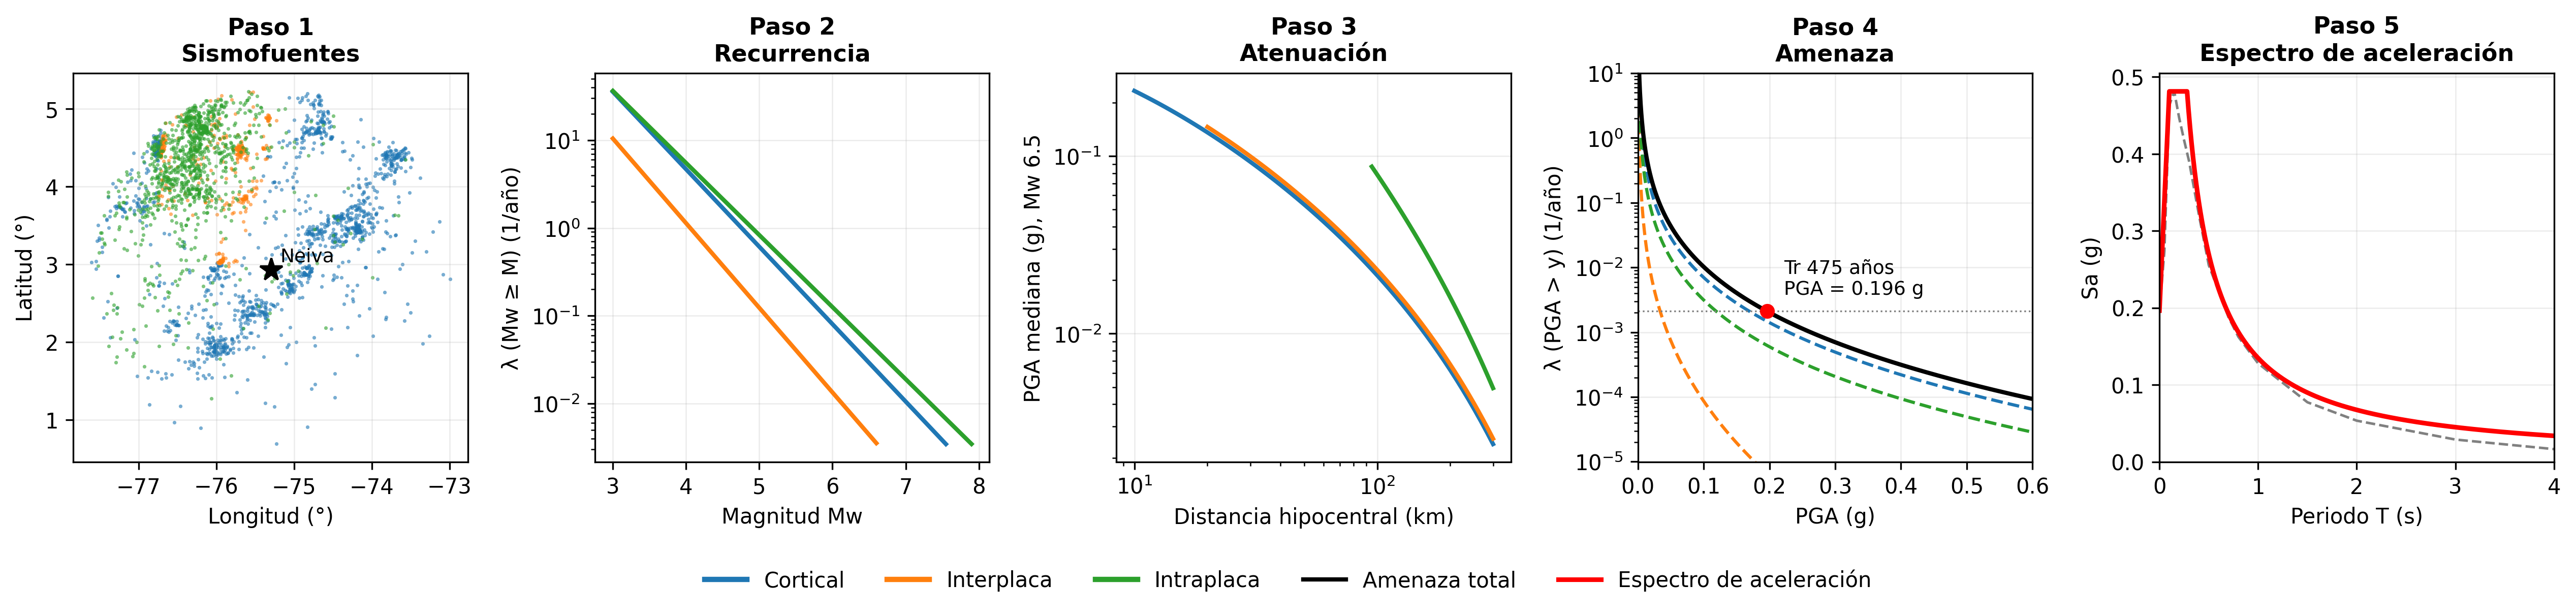
\includegraphics[width=\linewidth]{../figuras/metodologia_cinco_pasos.png}
    \caption[Pasos del análisis de amenaza sísmica]{Pasos del análisis de amenaza sísmica. Cada panel muestra el resultado de un paso con los datos de este estudio.}
    \label{fig:metodologia}
\end{figure}

\section{Paso 1: caracterización de sismofuentes}

Se usó el catálogo de sismicidad del Servicio Geológico Colombiano
\parencite{sgcCatalogoSismicidad} en un radio regional de 260 km alrededor
del sitio. Cada sismo se asoció a una de tres fuentes según su ubicación,
profundidad y relación con la placa de Nazca y las fallas corticales
\parencite{criteriosAsociacionNeiva2026}. El catálogo clasificado tiene
2\,691 sismos con $M_w\geq3.0$: 1\,308 corticales, 359 de subducción
interplaca y 1\,024 de subducción intraplaca
(Figura~\ref{fig:fuentes-neiva}). El periodo de análisis es 1917--2025
(109 años).

\begin{figure}[H]
    \centering
    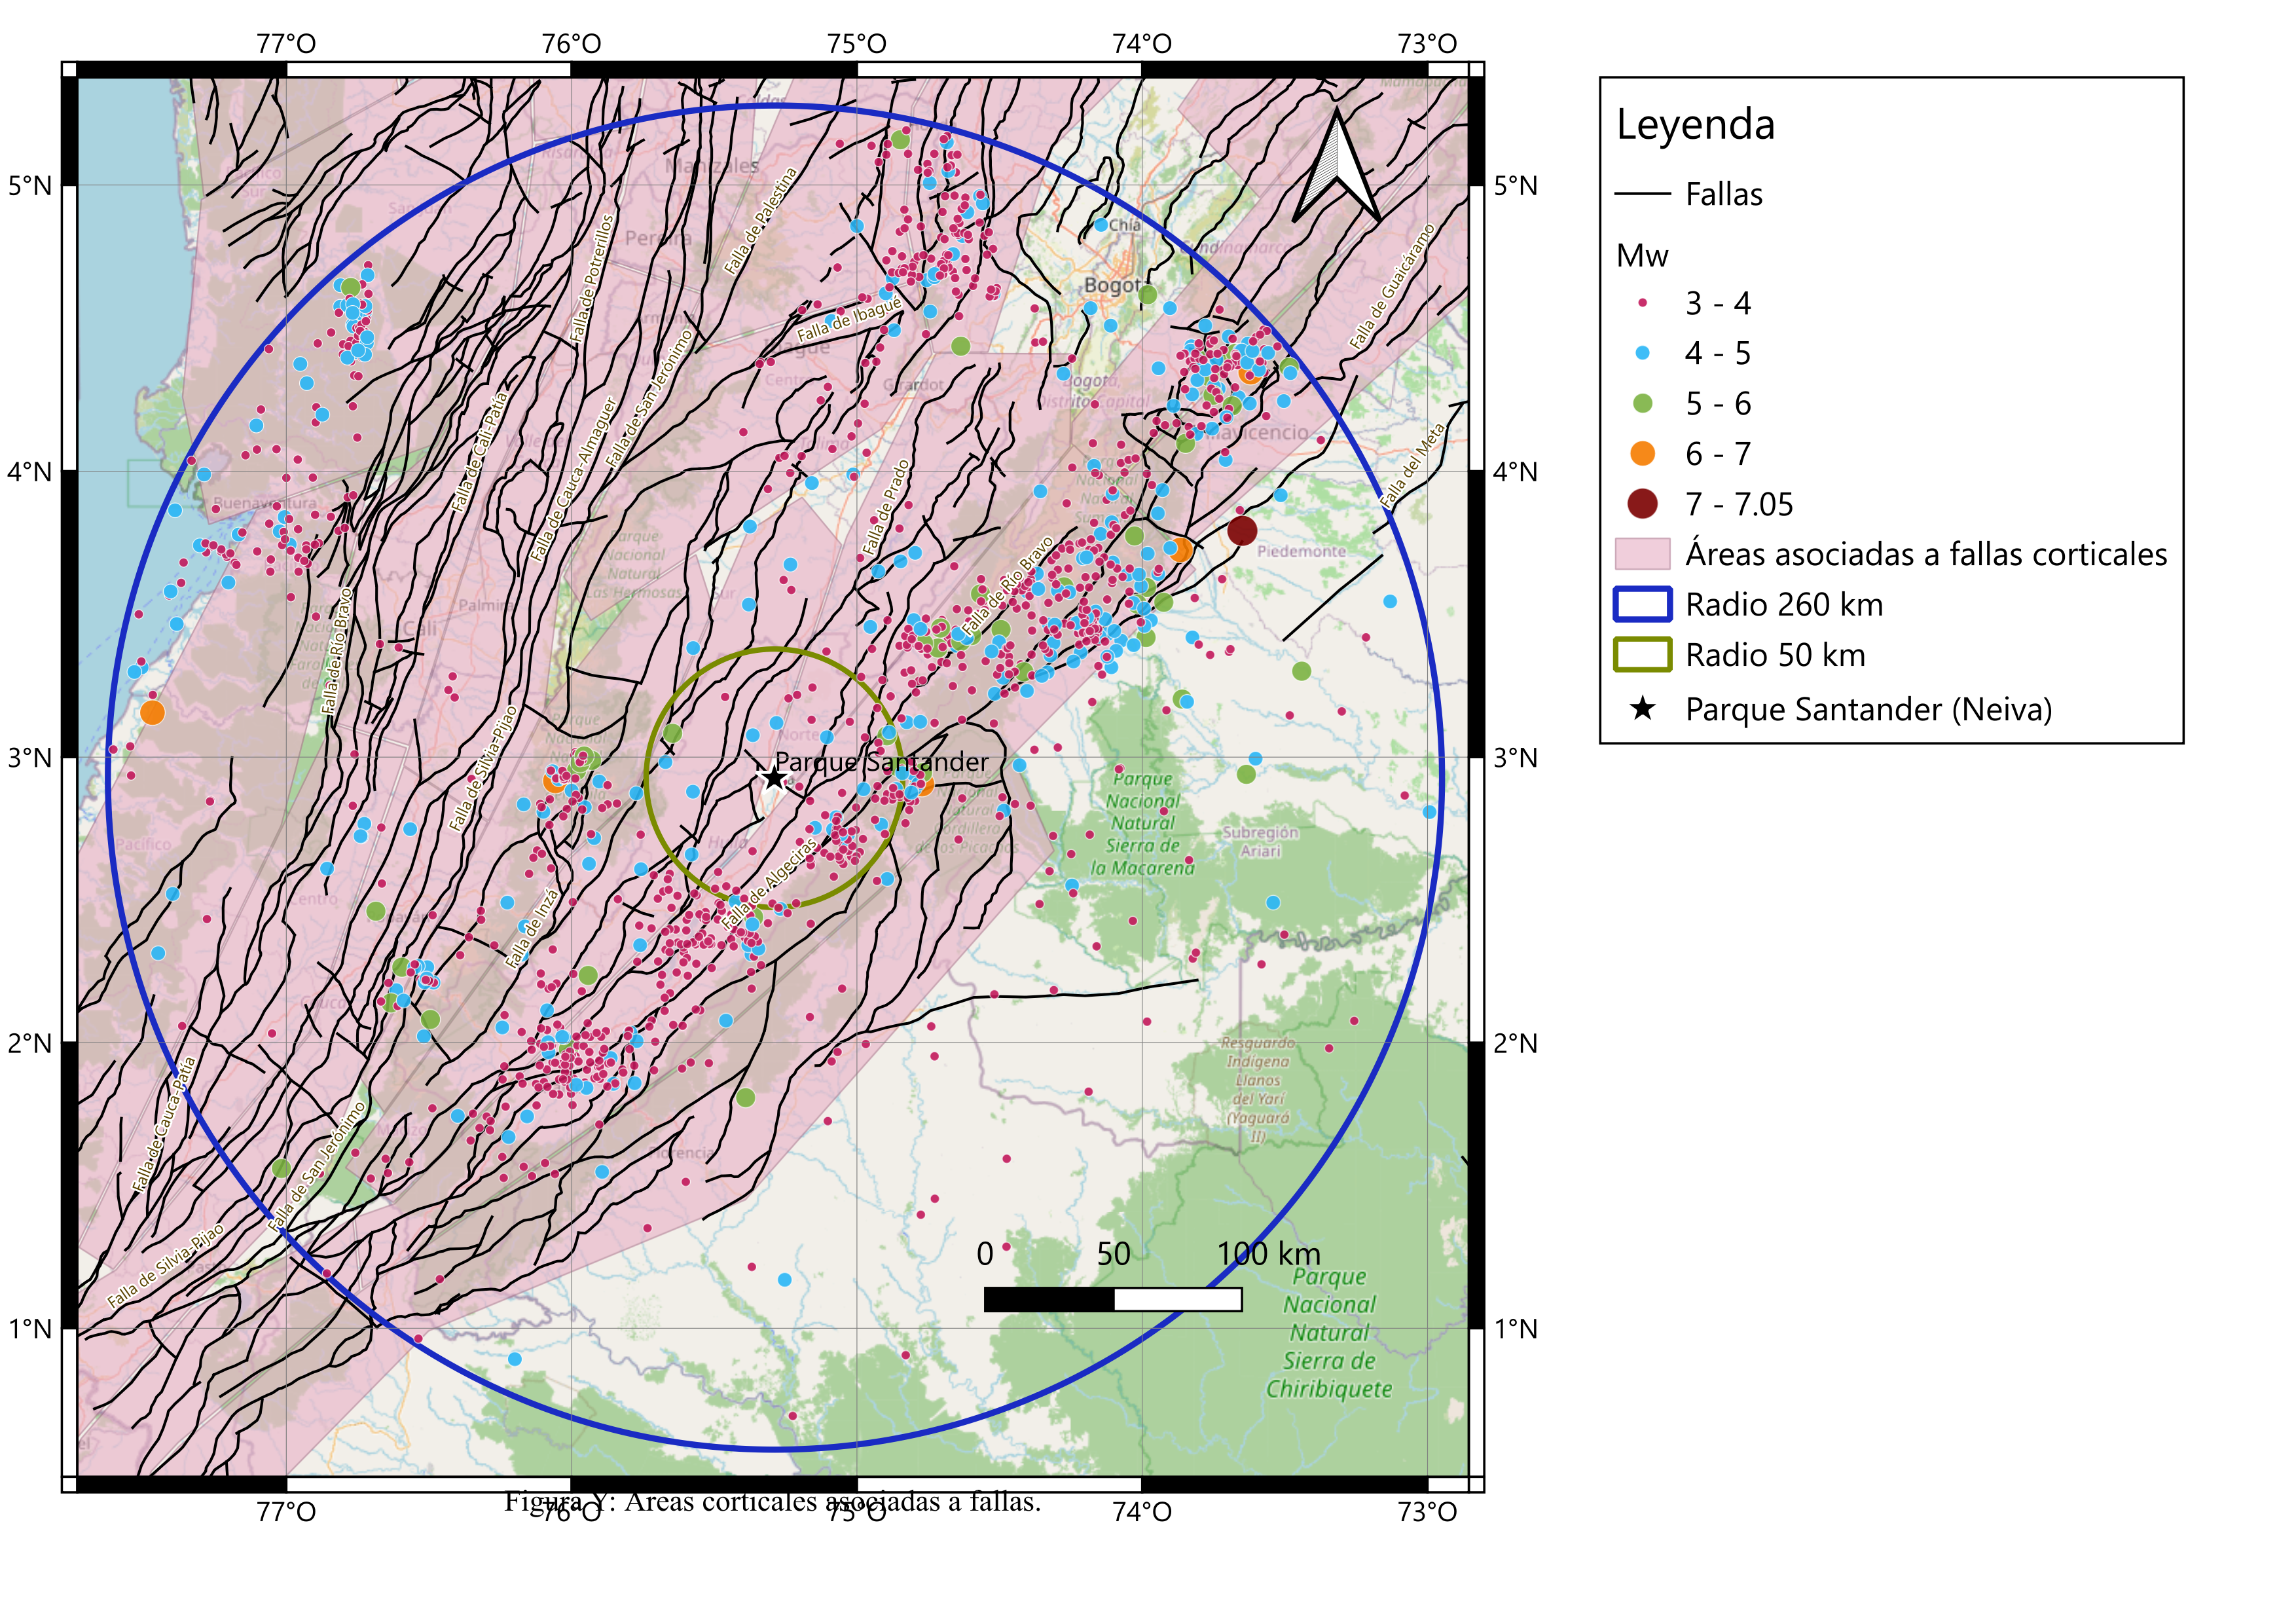
\includegraphics[width=0.62\linewidth,height=0.38\textheight,keepaspectratio]{../recursos/Qgis/datos/Figura_areas_corticales_fallas.png}
    \caption[Sismofuentes y fallas alrededor de Neiva]{Sismofuentes y fallas alrededor de Neiva. La sismicidad cortical rodea el sitio y la de subducción se concentra al noroccidente; el análisis usa el círculo de 260 km (el de 50 km es solo de referencia).}
    \label{fig:fuentes-neiva}
\end{figure}

\section{Paso 2: recurrencia sísmica}

\subsection{Completez del catálogo}

La red sismológica solo registra de forma completa los sismos pequeños desde
las últimas décadas. Por eso, para cada fuente e intervalo de magnitud se
buscó el año desde el cual el catálogo está completo. Para $M_w<5.0$ se usó
una regresión segmentada del número acumulado de sismos por año: el punto
de quiebre marca el inicio del periodo completo (con $R^2\geq0.90$ y al menos
10 años y 3 eventos por tramo). Para $M_w\geq5.0$ se usó todo el periodo
1917--2025. La tasa anual de cada intervalo es
\begin{equation*}
\lambda=\frac{N_{\mathrm{completo}}}{\Delta t_{\mathrm{completo}}},
\end{equation*}
donde $N_{\mathrm{completo}}$ es el número de sismos del intervalo dentro del
periodo completo y $\Delta t_{\mathrm{completo}}$ su duración en años.

\begin{figure}[H]
    \centering
    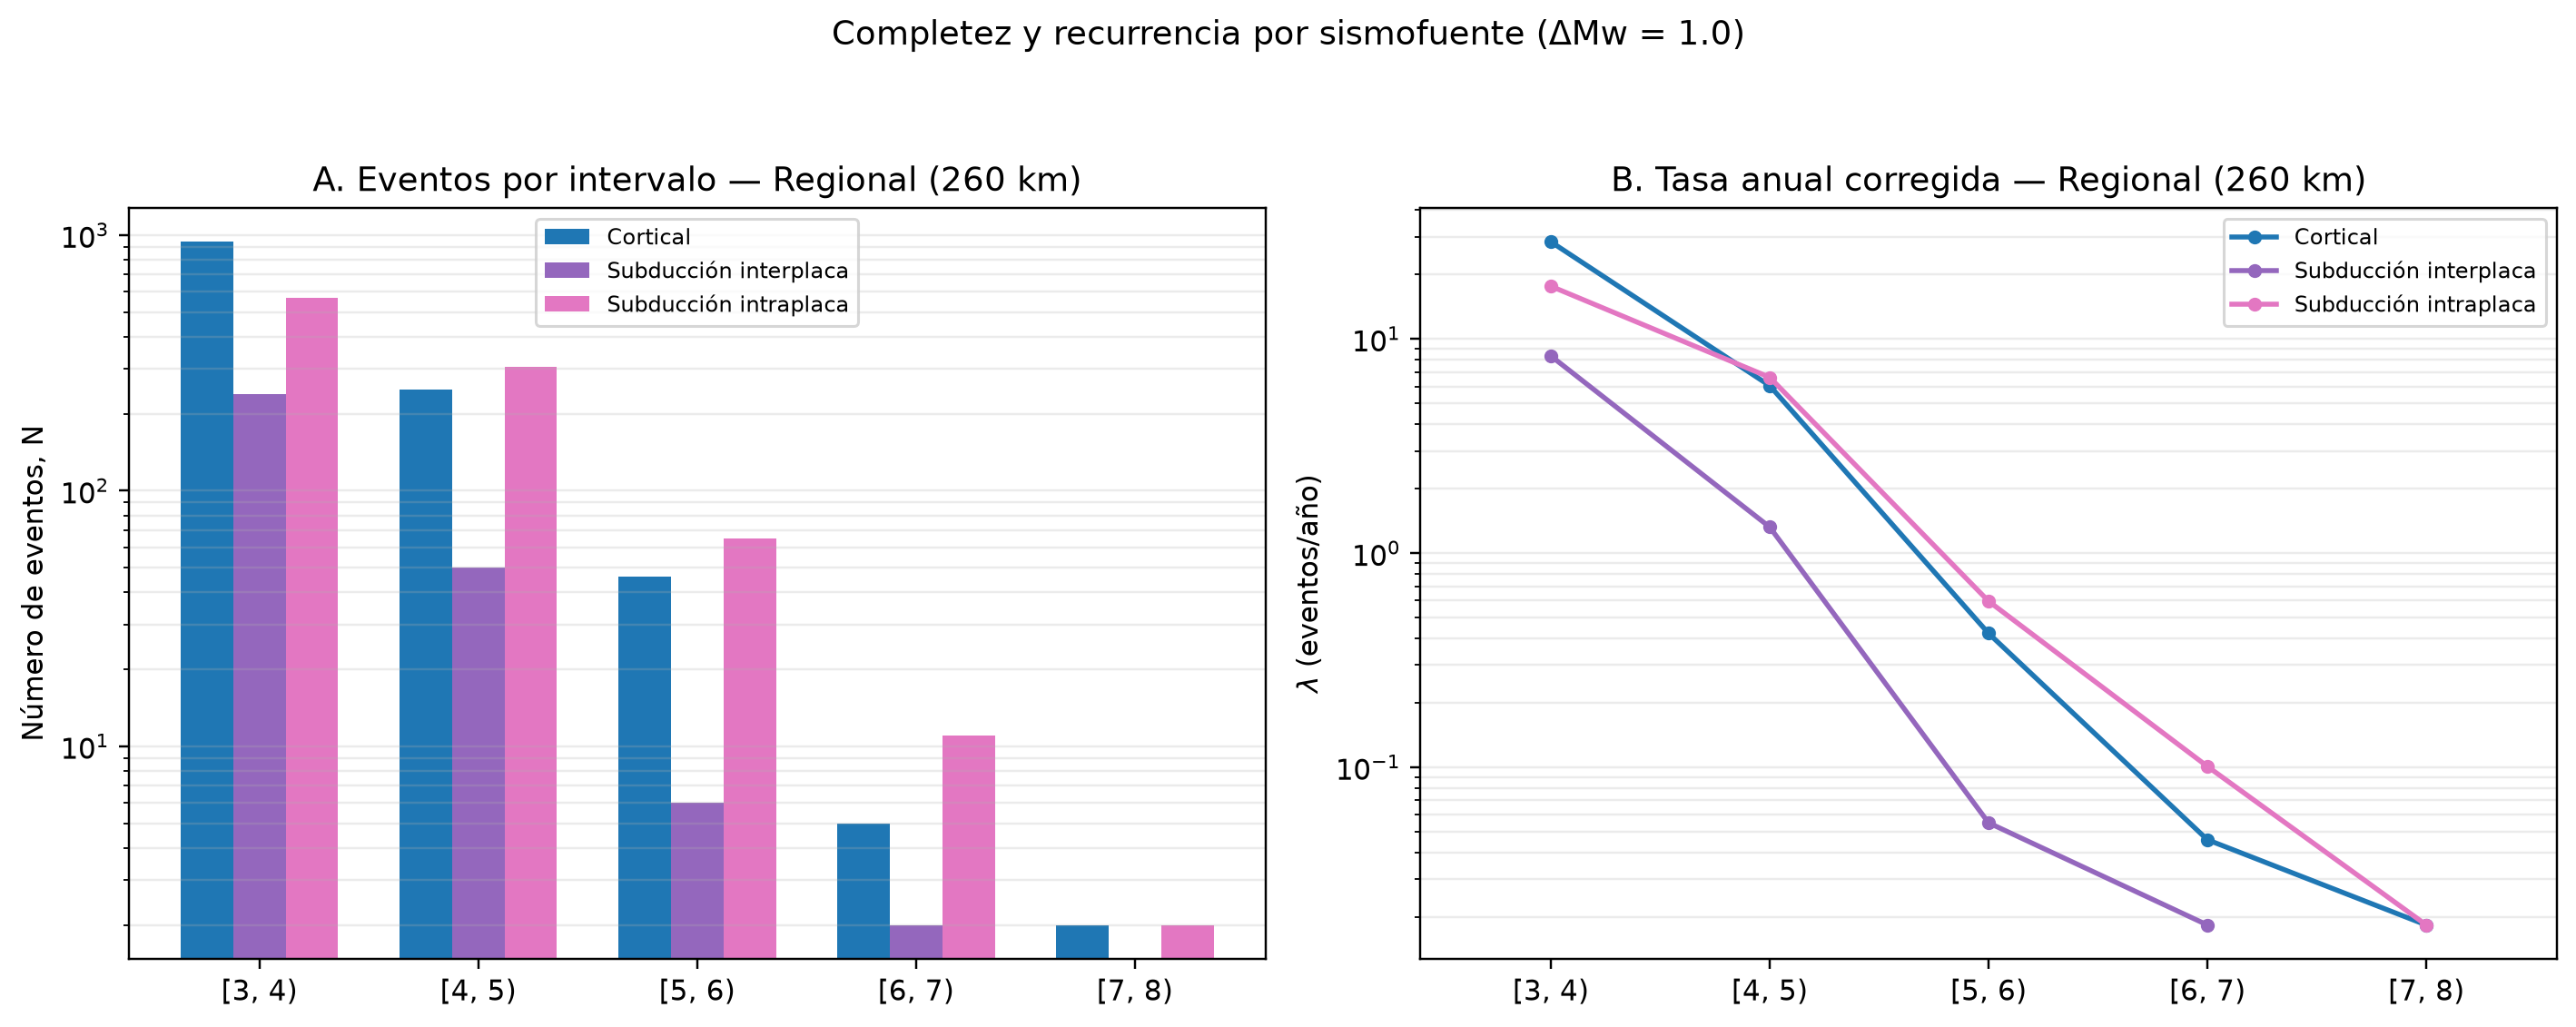
\includegraphics[width=0.89\linewidth]{../figuras/completez_recurrencia_fuentes_intervalos_1mw.png}
    \caption[Conteos y tasas anuales por fuente]{Conteos y tasas anuales por fuente. La fuente cortical domina en magnitudes bajas y la intraplaca en $M_w$ 5--7.}
    \label{fig:completez-regional}
\end{figure}

\begin{table}[H]
\centering
\customtablecaption{Tabla 1}{Completez y tasas anuales por fuente.}
\scriptsize
\begin{tabular}{llrrrrr}
\toprule
Sismofuente & Intervalo $M_w$ & $N$ & Inicio & $\Delta t$ (años) & $R^2$ & $\lambda$ (eventos/año) \\
\midrule
Cortical & $[3,4)$ & 941 & 1993 & 33 & 0.998 & 28.424 \\
Cortical & $[4,5)$ & 248 & 1987 & 39 & 0.980 & 6.051 \\
Cortical & $[5,6)$ & 46 & 1917 & 109 & -- & 0.422 \\
Cortical & $[6,7)$ & 5 & 1917 & 109 & -- & 0.046 \\
Cortical & $[7,8)$ & 2 & 1917 & 109 & -- & 0.018 \\
Subducción interplaca & $[3,4)$ & 239 & 1999 & 27 & 0.963 & 8.333 \\
Subducción interplaca & $[4,5)$ & 50 & 1992 & 34 & 0.977 & 1.324 \\
Subducción interplaca & $[5,6)$ & 6 & 1917 & 109 & -- & 0.055 \\
Subducción interplaca & $[6,7)$ & 2 & 1917 & 109 & -- & 0.018 \\
Subducción intraplaca & $[3,4)$ & 569 & 1994 & 32 & 0.996 & 17.625 \\
Subducción intraplaca & $[4,5)$ & 306 & 1984 & 42 & 0.994 & 6.619 \\
Subducción intraplaca & $[5,6)$ & 65 & 1917 & 109 & -- & 0.596 \\
Subducción intraplaca & $[6,7)$ & 11 & 1917 & 109 & -- & 0.101 \\
Subducción intraplaca & $[7,8)$ & 2 & 1917 & 109 & -- & 0.018 \\
\bottomrule
\end{tabular}
\end{table}

Los sismos $M_w$ 3--4 están completos desde 1993--1999 y los $M_w$ 4--5
desde 1984--1992, según la fuente. La fuente cortical es la más activa en
magnitudes bajas (28.4 sismos/año de $M_w$ 3--4) y la intraplaca en
magnitudes altas (0.60 sismos/año de $M_w$ 5--6, frente a 0.42 de la
cortical).

\subsection{Curvas de Gutenberg--Richter}

Con las tasas anteriores se ajustó, para cada fuente, la relación de
Gutenberg--Richter \parencite{gutenbergRichter1944}:
\begin{equation*}
\log_{10}\lambda(M_w\geq M)=a-bM,
\end{equation*}
donde $\lambda(M_w\geq M)$ es el número de sismos por año con magnitud mayor
o igual a $M$, $a$ indica qué tan activa es la fuente y $b$ cuántos sismos
pequeños hay por cada sismo grande. Los valores de $a$ y $b$ son resultado
de la regresión con umbrales de $M_w=3.0$ a 7.0 (Tabla~\ref{tab:gr-regional}).

\begin{table}[H]
\centering
\customtablecaption{Tabla 2}{Parámetros de Gutenberg--Richter por fuente.}
\label{tab:gr-regional}
\scriptsize
\begin{tabular}{lrrrr}
\toprule
Sismofuente & $a$ & $b$ & $R^2$ & $M_{w,\max}$ adoptada \\
\midrule
Cortical & 4.197 & 0.882 & 0.987 & 7.55 \\
Subducción interplaca & 3.911 & 0.964 & 0.976 & 6.60 \\
Subducción intraplaca & 4.025 & 0.821 & 0.992 & 7.90 \\
\bottomrule
\end{tabular}
\end{table}

\begin{figure}[H]
    \centering
    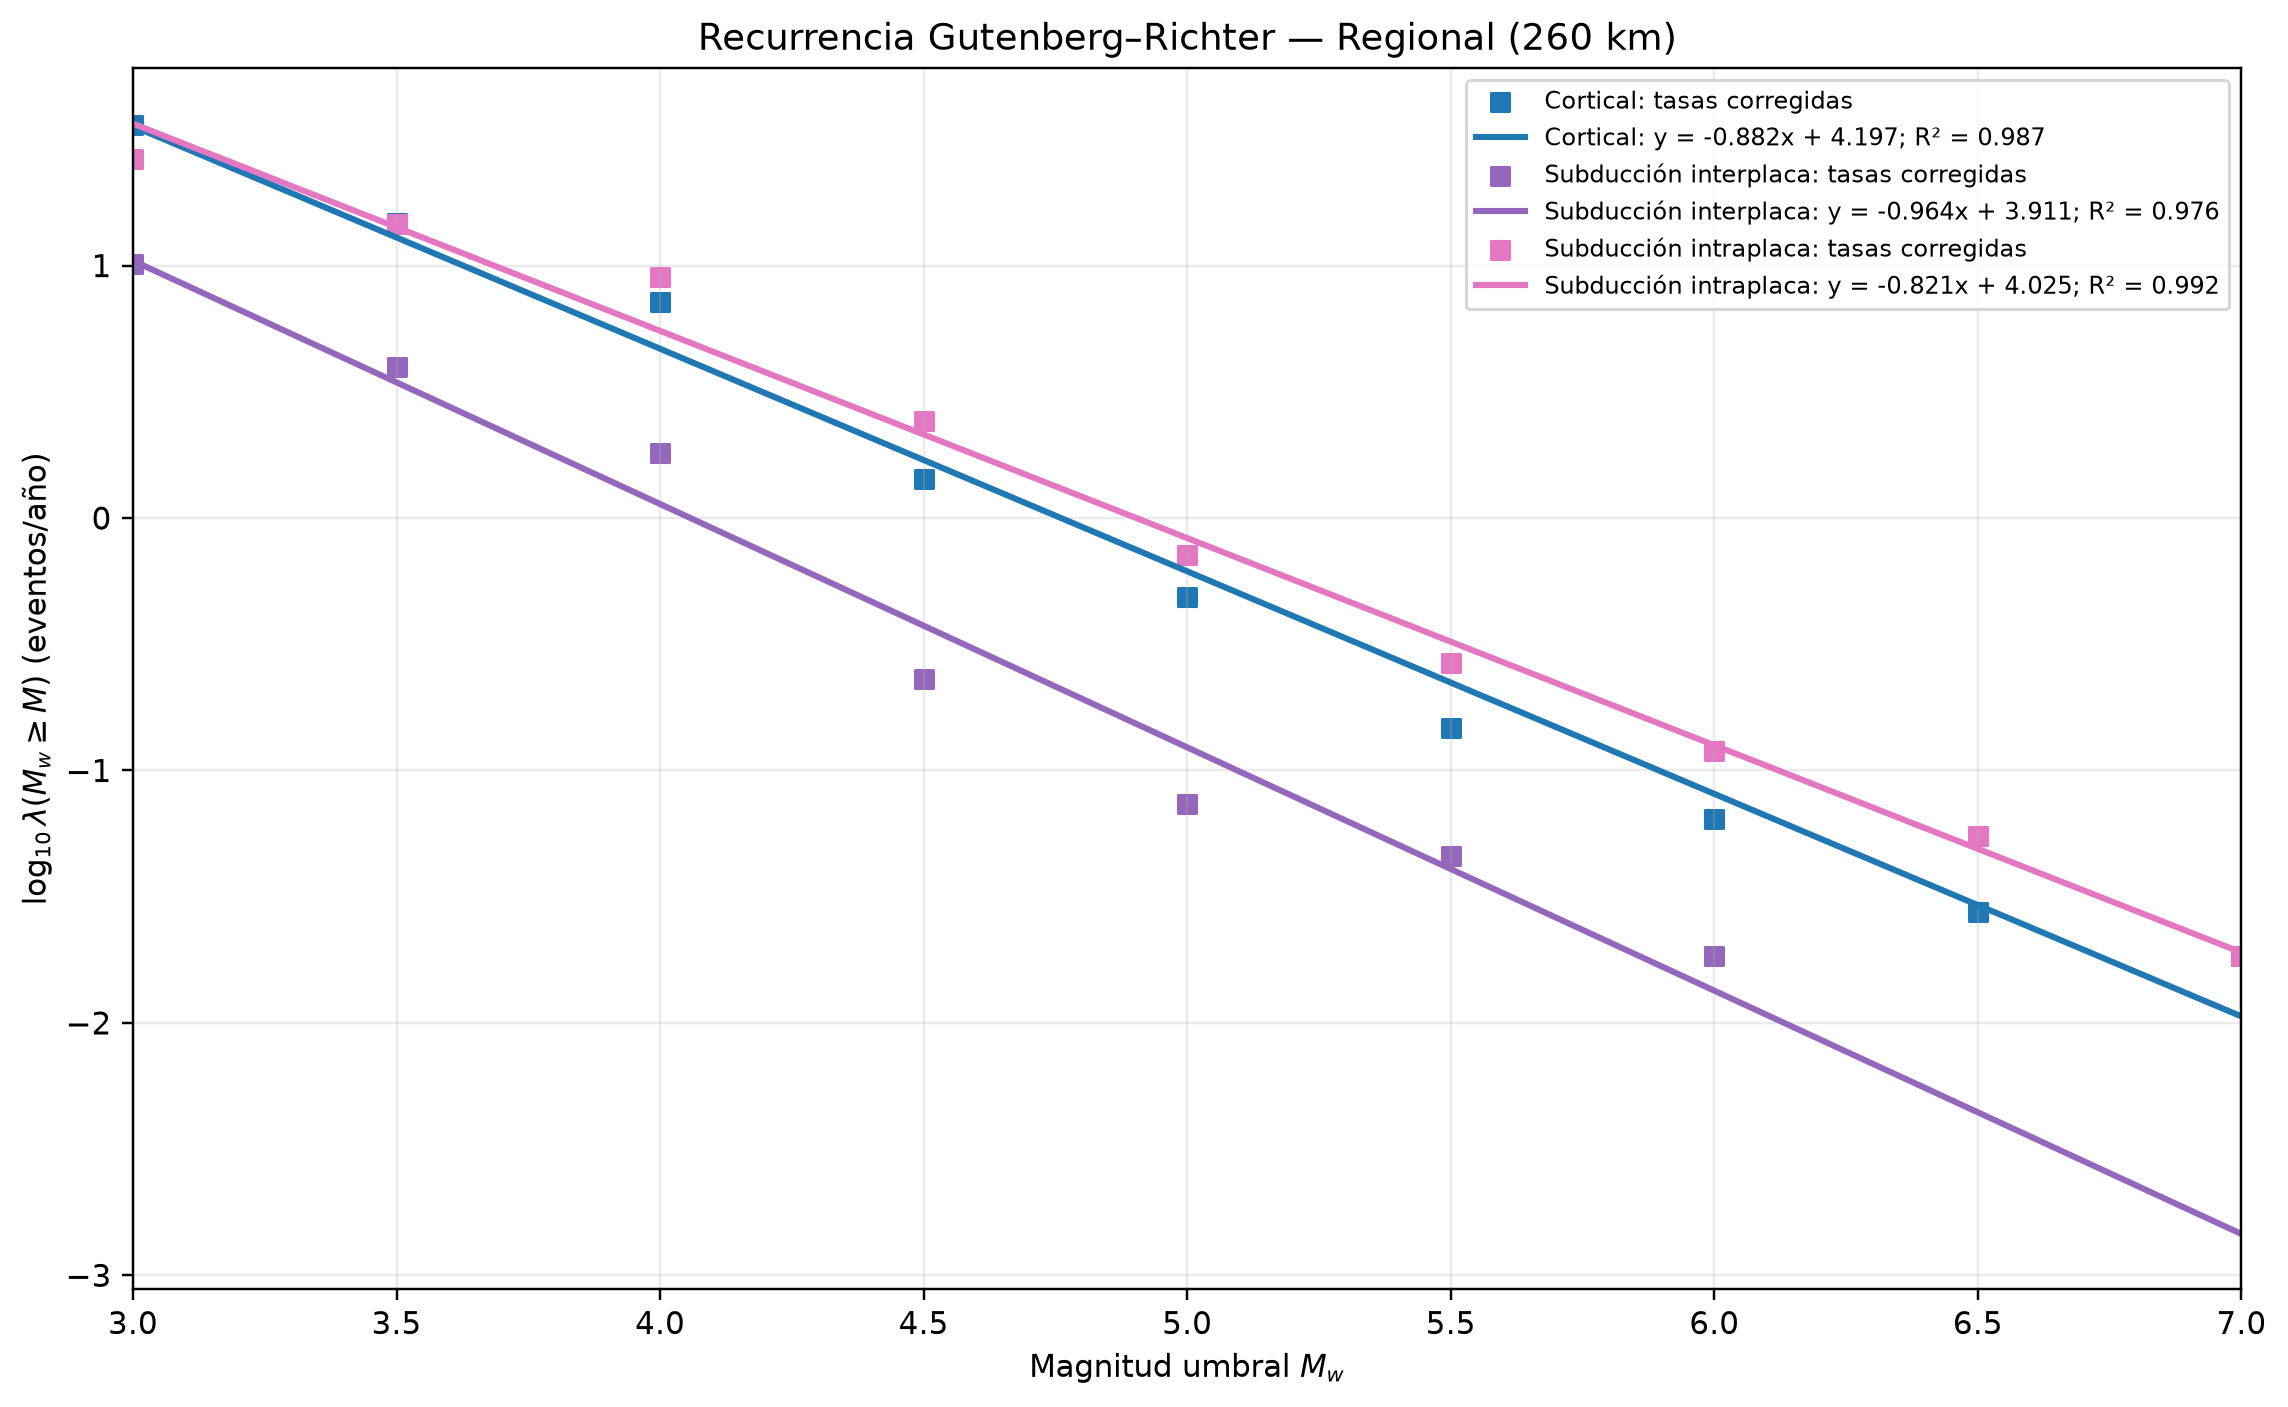
\includegraphics[width=0.72\linewidth]{../figuras/curvas_recurrencia_sismofuentes_regional.png}
    \caption[Curvas de recurrencia por fuente]{Curvas de recurrencia por fuente. La intraplaca tiene la menor pendiente ($b=0.821$), es decir, la mayor proporción de sismos grandes.}
    \label{fig:recurrencia-regional}
\end{figure}

Para el Paso 4 la recta se limita entre una magnitud mínima y una máxima
(Gutenberg--Richter truncado):
\begin{itemize}
    \item \textbf{$M_{w,\min}=3.0$}, la menor magnitud usada al depurar el
    catálogo y asociar los sismos a las fuentes.
    \item \textbf{$M_{w,\max}$ = mayor magnitud registrada + 0.5}
    (Tabla~\ref{tab:gr-regional}). Las mayores registradas son 7.05
    (cortical), 6.10 (interplaca) y 7.40 (intraplaca). Se suma 0.5 porque en
    109 años es poco probable haber registrado el sismo más grande posible de
    cada fuente.
\end{itemize}
No se usó el modelo característico \parencite{youngs1985} porque necesita
datos geológicos de las fallas (tasas de deslizamiento y magnitudes máximas)
que no están disponibles para estas fuentes regionales.

\section{Paso 3: atenuación del movimiento}

Se adoptó la ecuación de Zhao et al. (2006) \parencite{zhao2006} porque tiene
términos propios para los tres tipos de fuente de Neiva y un término de
profundidad, necesario para los sismos intraplaca, que ocurren a unos
100 km de profundidad:
\begin{equation*}
\ln Y=aM_w+bX-\ln\!\left[X+c\,e^{dM_w}\right]+e\,(h-h_c)\,\delta_h
+F_R+S_I+S_S+S_{SL}\ln X+C_k,
\end{equation*}
donde:
\begin{itemize}
    \item $Y$: PGA mediana en cm/s$^2$.
    \item $M_w$: magnitud momento.
    \item $X$: distancia hipocentral en km, $X=\sqrt{X_{\mathrm{epi}}^2+h^2}$,
    con $X_{\mathrm{epi}}$ la distancia epicentral al sitio.
    \item $h$: profundidad focal en km (máximo 125 km); $h_c=15$ km;
    $\delta_h=1$ si $h\geq h_c$ y 0 si no.
    \item $a,b,c,d,e$: coeficientes de regresión.
    \item $F_R$, $S_I$, $S_S$, $S_{SL}$: términos de la fuente cortical
    inversa, interplaca e intraplaca; cada sismo usa solo el de su fuente.
    \item $C_k$: término de sitio.
\end{itemize}
Todos los coeficientes se tomaron de las Tablas 4 y 5 de Zhao et al. (2006)
para PGA (Tabla~3).

\begin{table}[H]
\centering
\customtablecaption{Tabla 3}{Coeficientes de Zhao et al. (2006) para PGA en roca.}
\scriptsize
\begin{tabular}{lrl}
\toprule
Parámetro & Valor & Uso \\
\midrule
$a$ & 1.101 & Magnitud \\
$b$ & $-0.00564$ & Distancia \\
$c$ & 0.0055 & Distancia ajustada \\
$d$ & 1.080 & Distancia ajustada \\
$e$ & 0.01412 & Profundidad \\
$F_R$ & 0 & Cortical (coeficiente 0.251 desactivado) \\
$S_I$ & 0.000 & Interplaca \\
$S_S$ & 2.607 & Intraplaca \\
$S_{SL}$ & $-0.528$ & Intraplaca \\
$C_k=C_1$ & 1.111 & Roca, Clase I \\
$\sigma_{\ln}$ & 0.723 & Desviación estándar total \\
\bottomrule
\end{tabular}
\end{table}

Las decisiones adoptadas son:
\begin{itemize}
    \item \textbf{Distancia hipocentral.} Zhao mide la distancia a la ruptura
    y, cuando no hay modelo de falla, usa la hipocentral. Además, representa
    el recorrido de las ondas desde el foco: un sismo intraplaca puede tener
    el epicentro cerca de Neiva y estar a más de 100 km del sitio.
    \item \textbf{Sitio en roca, Clase I de Zhao} ($V_{S30}>600$ m/s,
    $C_1=1.111$). Es la condición de referencia para el análisis de respuesta
    de sitio de la siguiente etapa.
    \item \textbf{$F_R=0$.} El catálogo no tiene mecanismos focales para
    asignar falla inversa a los sismos corticales, y el sistema de fallas
    cercano, Algeciras--Garzón, es principalmente de rumbo.
\end{itemize}

Las Figuras~\ref{fig:atenuacion-cortical}--\ref{fig:atenuacion-intraplaca}
muestran el resultado. A igual magnitud y distancia, la intraplaca da PGA
mayores que la cortical: para un sismo a 95 km de profundidad y 130 km de
distancia, los términos de profundidad y $S_S$ multiplican la PGA por cerca
de 3.

\begin{figure}[H]
    \centering
    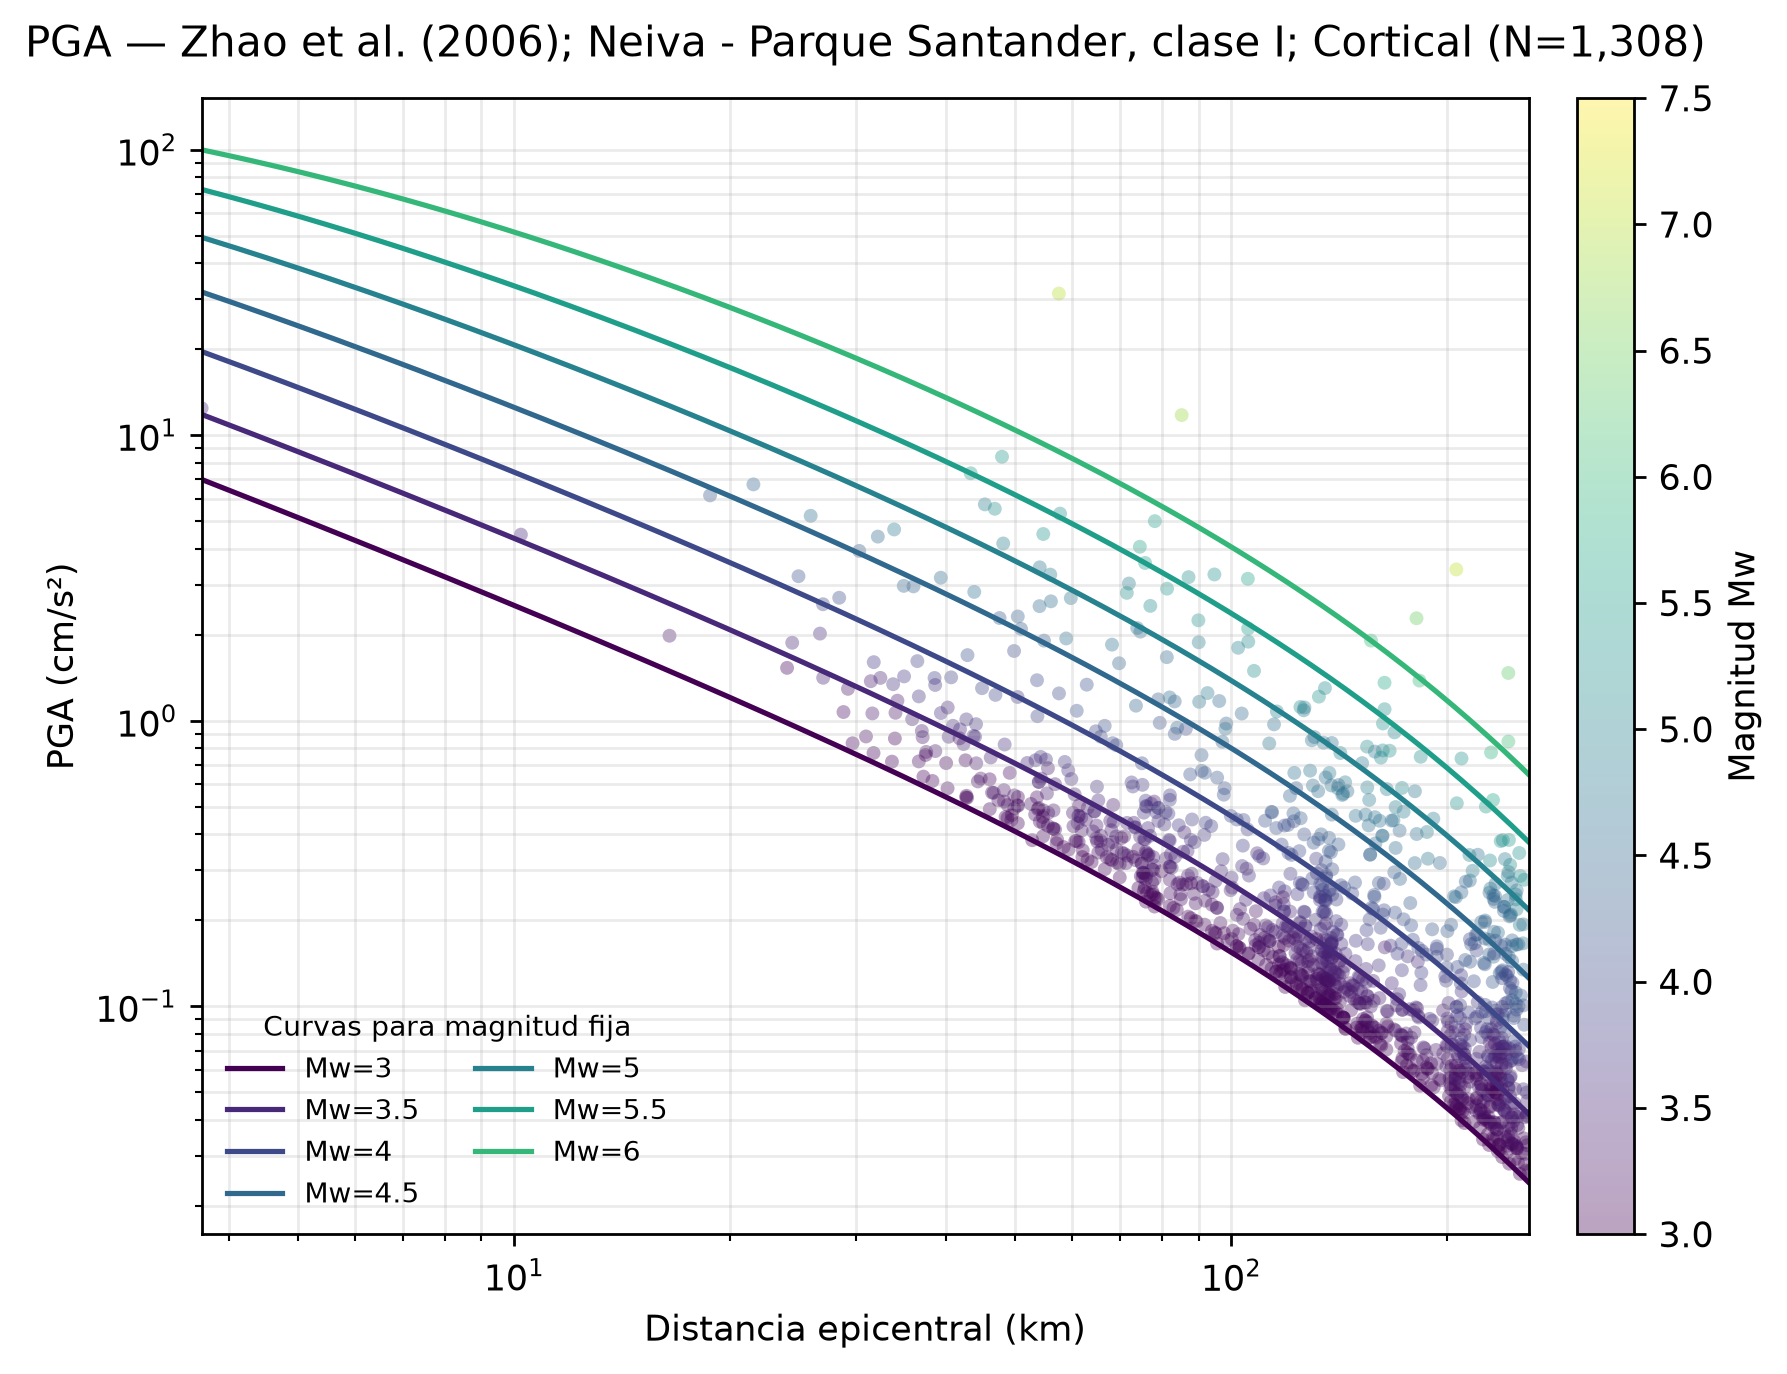
\includegraphics[width=0.64\linewidth]{../figuras/curvas_atenuacion_neiva_pga_cortical_logx.png}
    \caption[Atenuación de PGA, fuente cortical]{Atenuación de PGA, fuente cortical. Es la fuente con los sismos más cercanos al sitio.}
    \label{fig:atenuacion-cortical}
\end{figure}

\begin{figure}[H]
    \centering
    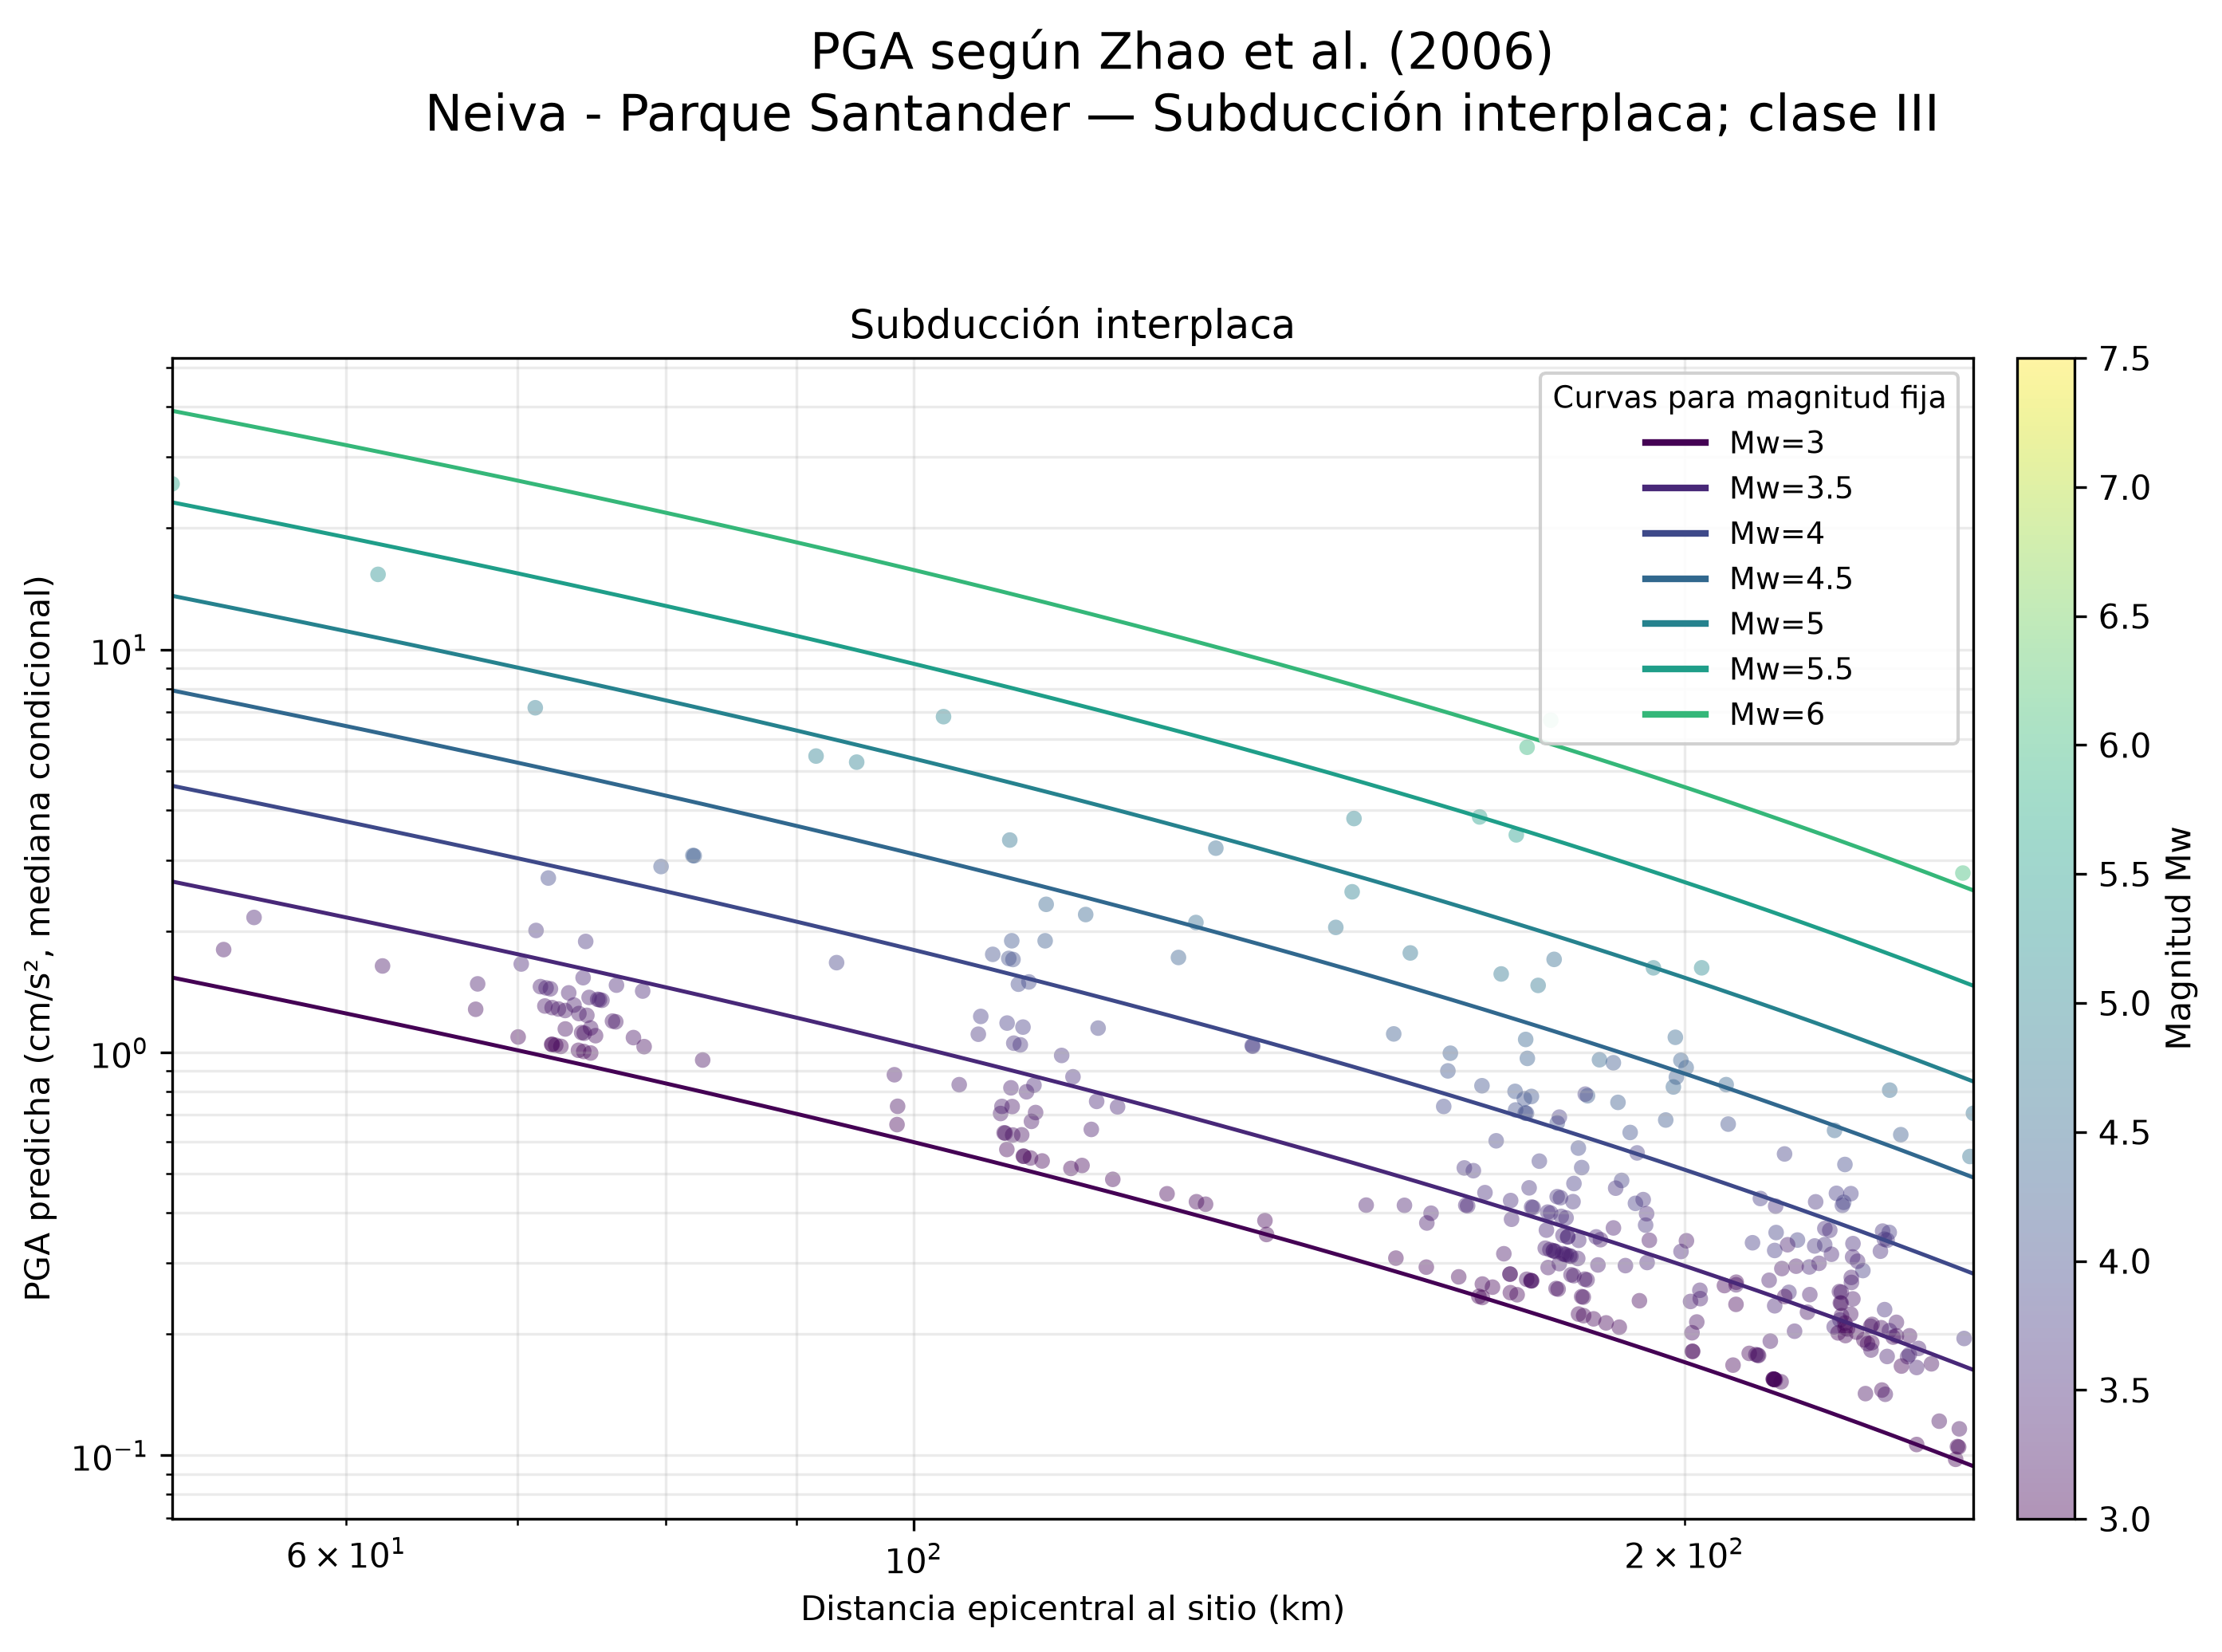
\includegraphics[width=0.64\linewidth]{../figuras/curvas_atenuacion_neiva_pga_interplaca_logx.png}
    \caption[Atenuación de PGA, subducción interplaca]{Atenuación de PGA, subducción interplaca. Los sismos están lejos del sitio y producen aceleraciones bajas.}
    \label{fig:atenuacion-interplaca}
\end{figure}

\begin{figure}[H]
    \centering
    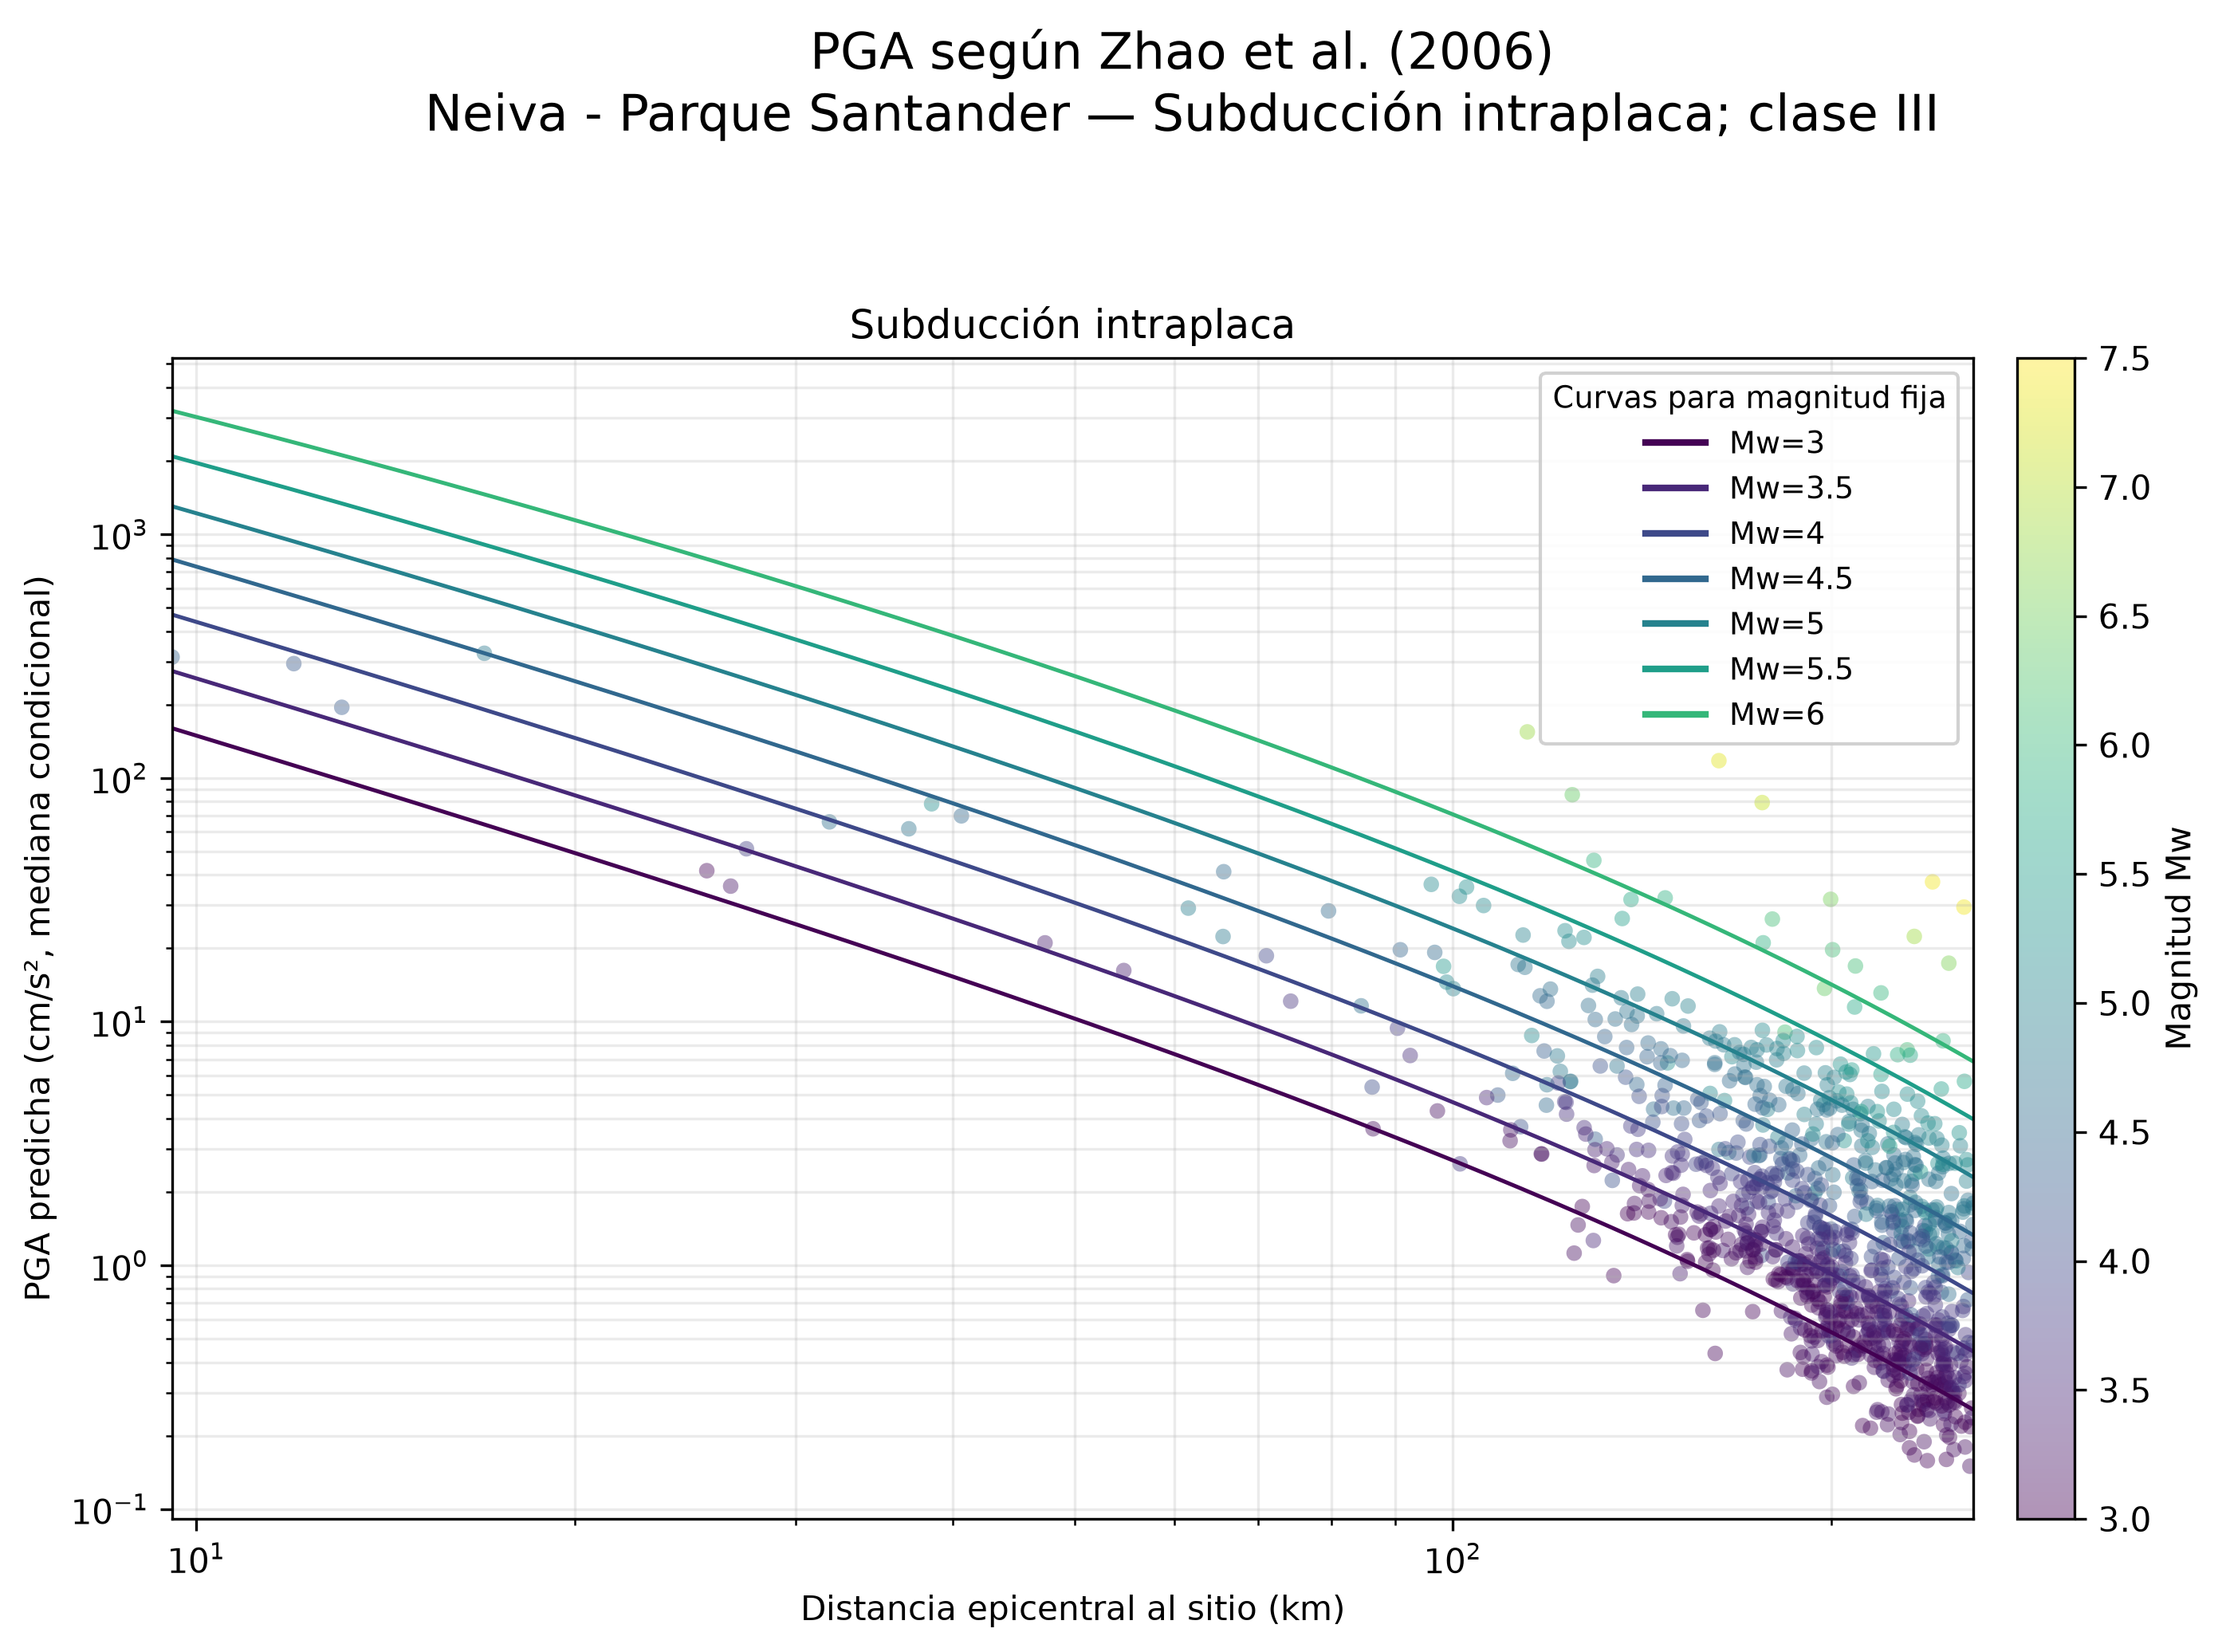
\includegraphics[width=0.64\linewidth]{../figuras/curvas_atenuacion_neiva_pga_intraplaca_logx.png}
    \caption[Atenuación de PGA, subducción intraplaca]{Atenuación de PGA, subducción intraplaca. Por los términos de profundidad y $S_S$, a igual distancia da PGA mayores que la cortical.}
    \label{fig:atenuacion-intraplaca}
\end{figure}

\section{Paso 4: amenaza sísmica}

\subsection{Curva de amenaza}

La tasa anual con que se supera un nivel de PGA $y$ se obtiene sumando, para
cada fuente $i$ y cada intervalo de magnitud $k$, la tasa de sismos por la
probabilidad de que produzcan más de $y$:
\begin{equation*}
\lambda(\mathrm{PGA}>y)=\sum_i\sum_k\Delta\nu_{i,k}\,
\frac{1}{N_i}\sum_{j=1}^{N_i}P\!\left(\mathrm{PGA}>y\mid M_k,X_{i,j},h_{i,j}\right),
\qquad
\Delta\nu_{i,k}=10^{a_i-b_iM_k}-10^{a_i-b_iM_{k+1}},
\end{equation*}
donde:
\begin{itemize}
    \item $\Delta\nu_{i,k}$: tasa anual de sismos de la fuente $i$ con
    magnitud entre $M_k$ y $M_{k+1}$ (intervalos de 0.025), con $a_i$ y
    $b_i$ de la Tabla~\ref{tab:gr-regional}.
    \item $X_{i,j}$, $h_{i,j}$: distancia hipocentral y profundidad de cada
    uno de los $N_i$ sismos del catálogo de la fuente; así la ubicación de
    los sismos futuros sigue la de los sismos registrados.
    \item $P(\cdot)$: probabilidad lognormal con la mediana de Zhao y
    $\sigma_{\ln}=0.723$ (Tabla~3). Se usa la desviación total porque el PGA
    real varía alrededor de la mediana; no incluirla subestima la amenaza.
\end{itemize}

\begin{figure}[H]
    \centering
    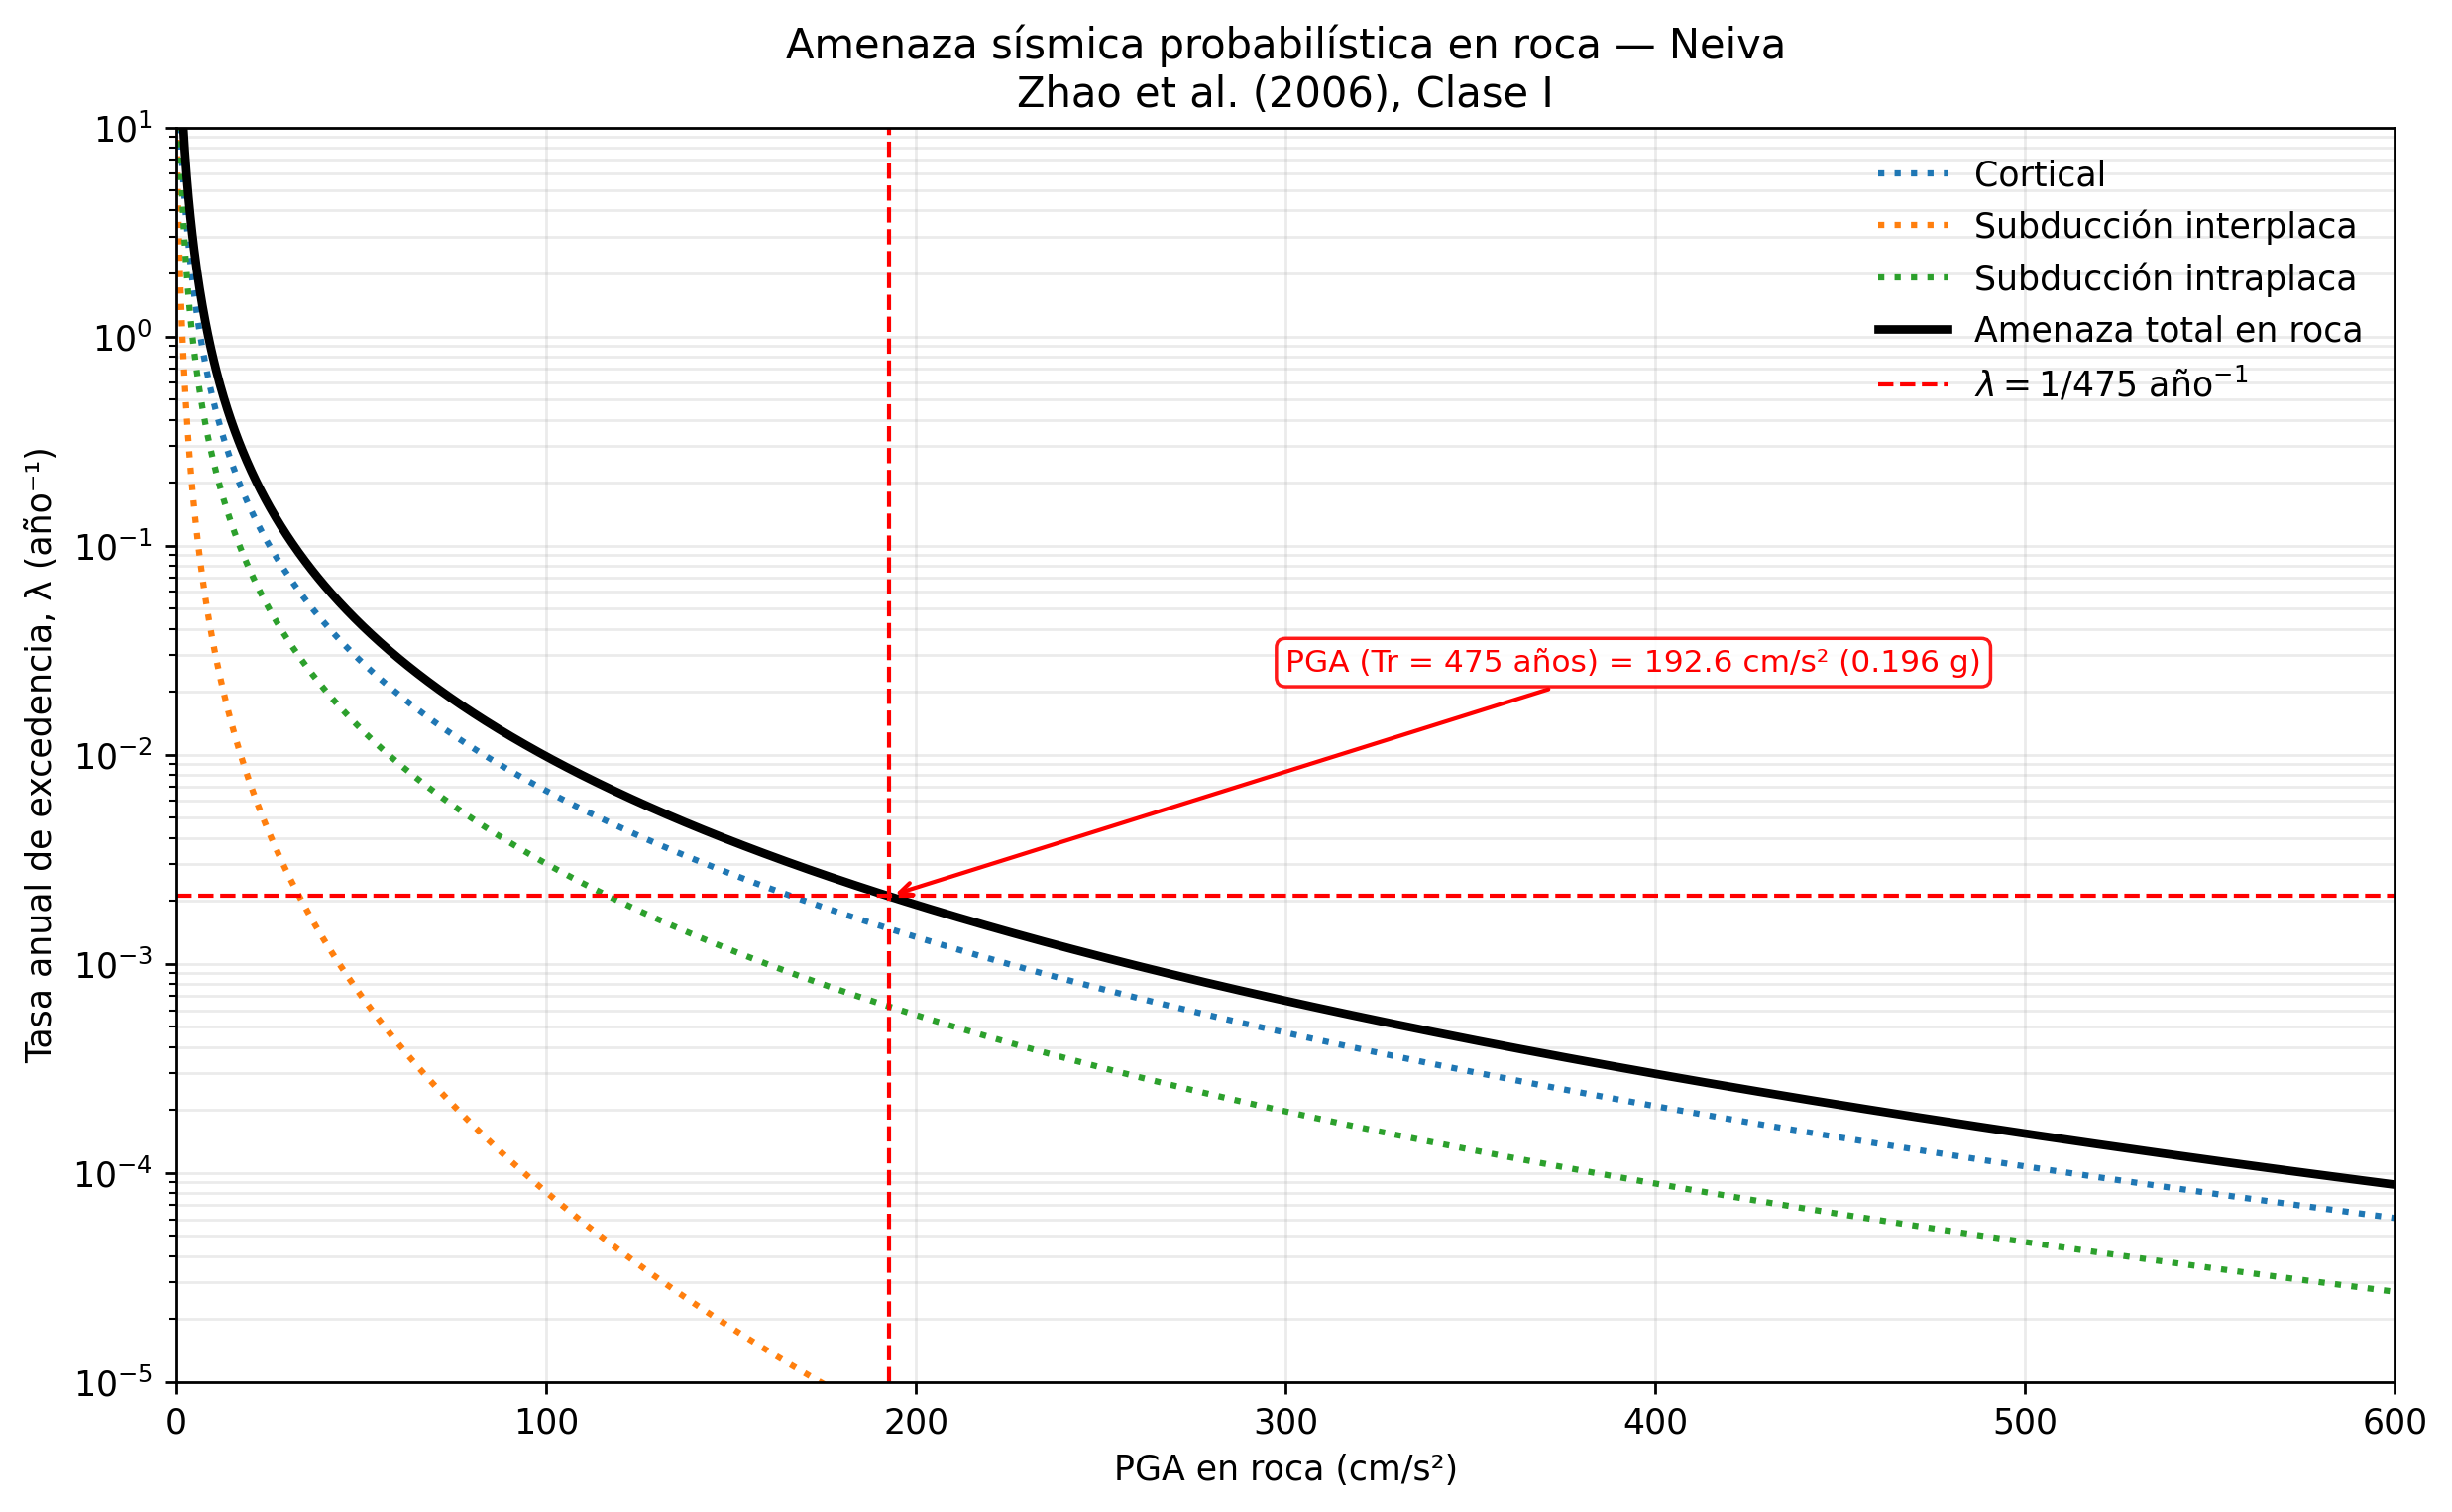
\includegraphics[width=0.74\linewidth]{../figuras/curva_amenaza_neiva_roca_pga_semi_log.png}
    \caption[Curva de amenaza sísmica en roca]{Curva de amenaza sísmica en roca. La fuente cortical aporta entre el 62 y el 70\% de la amenaza total, la intraplaca cerca del 30\% y la interplaca menos del 6\%.}
    \label{fig:amenaza-total-roca}
\end{figure}

El PGA de cada periodo de retorno $T_r$ es el valor donde la curva total
cruza $\lambda=1/T_r$ (Tabla~\ref{tab:pga-diseno-roca}). La probabilidad de
excedencia en 50 años es $1-e^{-50/T_r}$.

\begin{table}[H]
\centering
\customtablecaption{Tabla 4}{PGA en roca por periodo de retorno.}
\label{tab:pga-diseno-roca}
\scriptsize
\begin{tabular}{rrrrr}
\toprule
$T_r$ (años) & $\lambda$ (año$^{-1}$) & PGA (cm/s$^2$) & PGA (g) & Excedencia en 50 años \\
\midrule
100  & 0.010000 & 99.1  & 0.101 & 39\% \\
475  & 0.002105 & 192.6 & 0.196 & 10\% \\
975  & 0.001026 & 255.1 & 0.260 & 5\% \\
2475 & 0.000404 & 359.3 & 0.366 & 2\% \\
\bottomrule
\end{tabular}
\end{table}

Para 475 años el PGA en roca es \textbf{0.196 $g$}, el 79\% del $A_a=0.25$ de
la NSR-10 para Neiva \parencite{nsr10}. Como $M_{w,\max}$ no se puede acotar
con datos geológicos, se varió en $\pm0.5$: el PGA cambia cerca de un 10\%
(Tabla~\ref{tab:sensibilidad-pga}).

\begin{table}[H]
\centering
\customtablecaption{Tabla 5}{Sensibilidad del PGA de 475 años a $M_{w,\max}$.}
\label{tab:sensibilidad-pga}
\scriptsize
\begin{tabular}{lr}
\toprule
Caso & PGA (g) \\
\midrule
$M_{w,\max}$ adoptada & 0.196 \\
$M_{w,\max}-0.5$ (magnitudes registradas) & 0.177 \\
$M_{w,\max}+0.5$ & 0.213 \\
\bottomrule
\end{tabular}
\end{table}

Para PGA entre 0 y 100 cm/s$^2$, las curvas se resumen con ajustes
$\lambda=A\,e^{-B\,\mathrm{PGA}}$ (Tabla~\ref{tab:ajustes-exponenciales-amenaza}).
Son solo descriptivos: los PGA de la Tabla~\ref{tab:pga-diseno-roca} salen de
la curva calculada.

\begin{table}[H]
\centering
\customtablecaption{Tabla 6}{Ajustes exponenciales de las curvas de amenaza (0--100 cm/s$^2$).}
\label{tab:ajustes-exponenciales-amenaza}
\scriptsize
\begin{tabular}{lrrr}
\toprule
Sismofuente & $A$ (año$^{-1}$) & $B$ ((cm/s$^2$)$^{-1}$) & $R^2$ \\
\midrule
Cortical & 0.65275 & 0.05350 & 0.8395 \\
Subducción interplaca & 0.05325 & 0.07461 & 0.8629 \\
Subducción intraplaca & 0.35476 & 0.05580 & 0.8276 \\
Amenaza total & 1.05965 & 0.05480 & 0.8325 \\
\bottomrule
\end{tabular}
\end{table}

\begin{figure}[H]
    \centering
    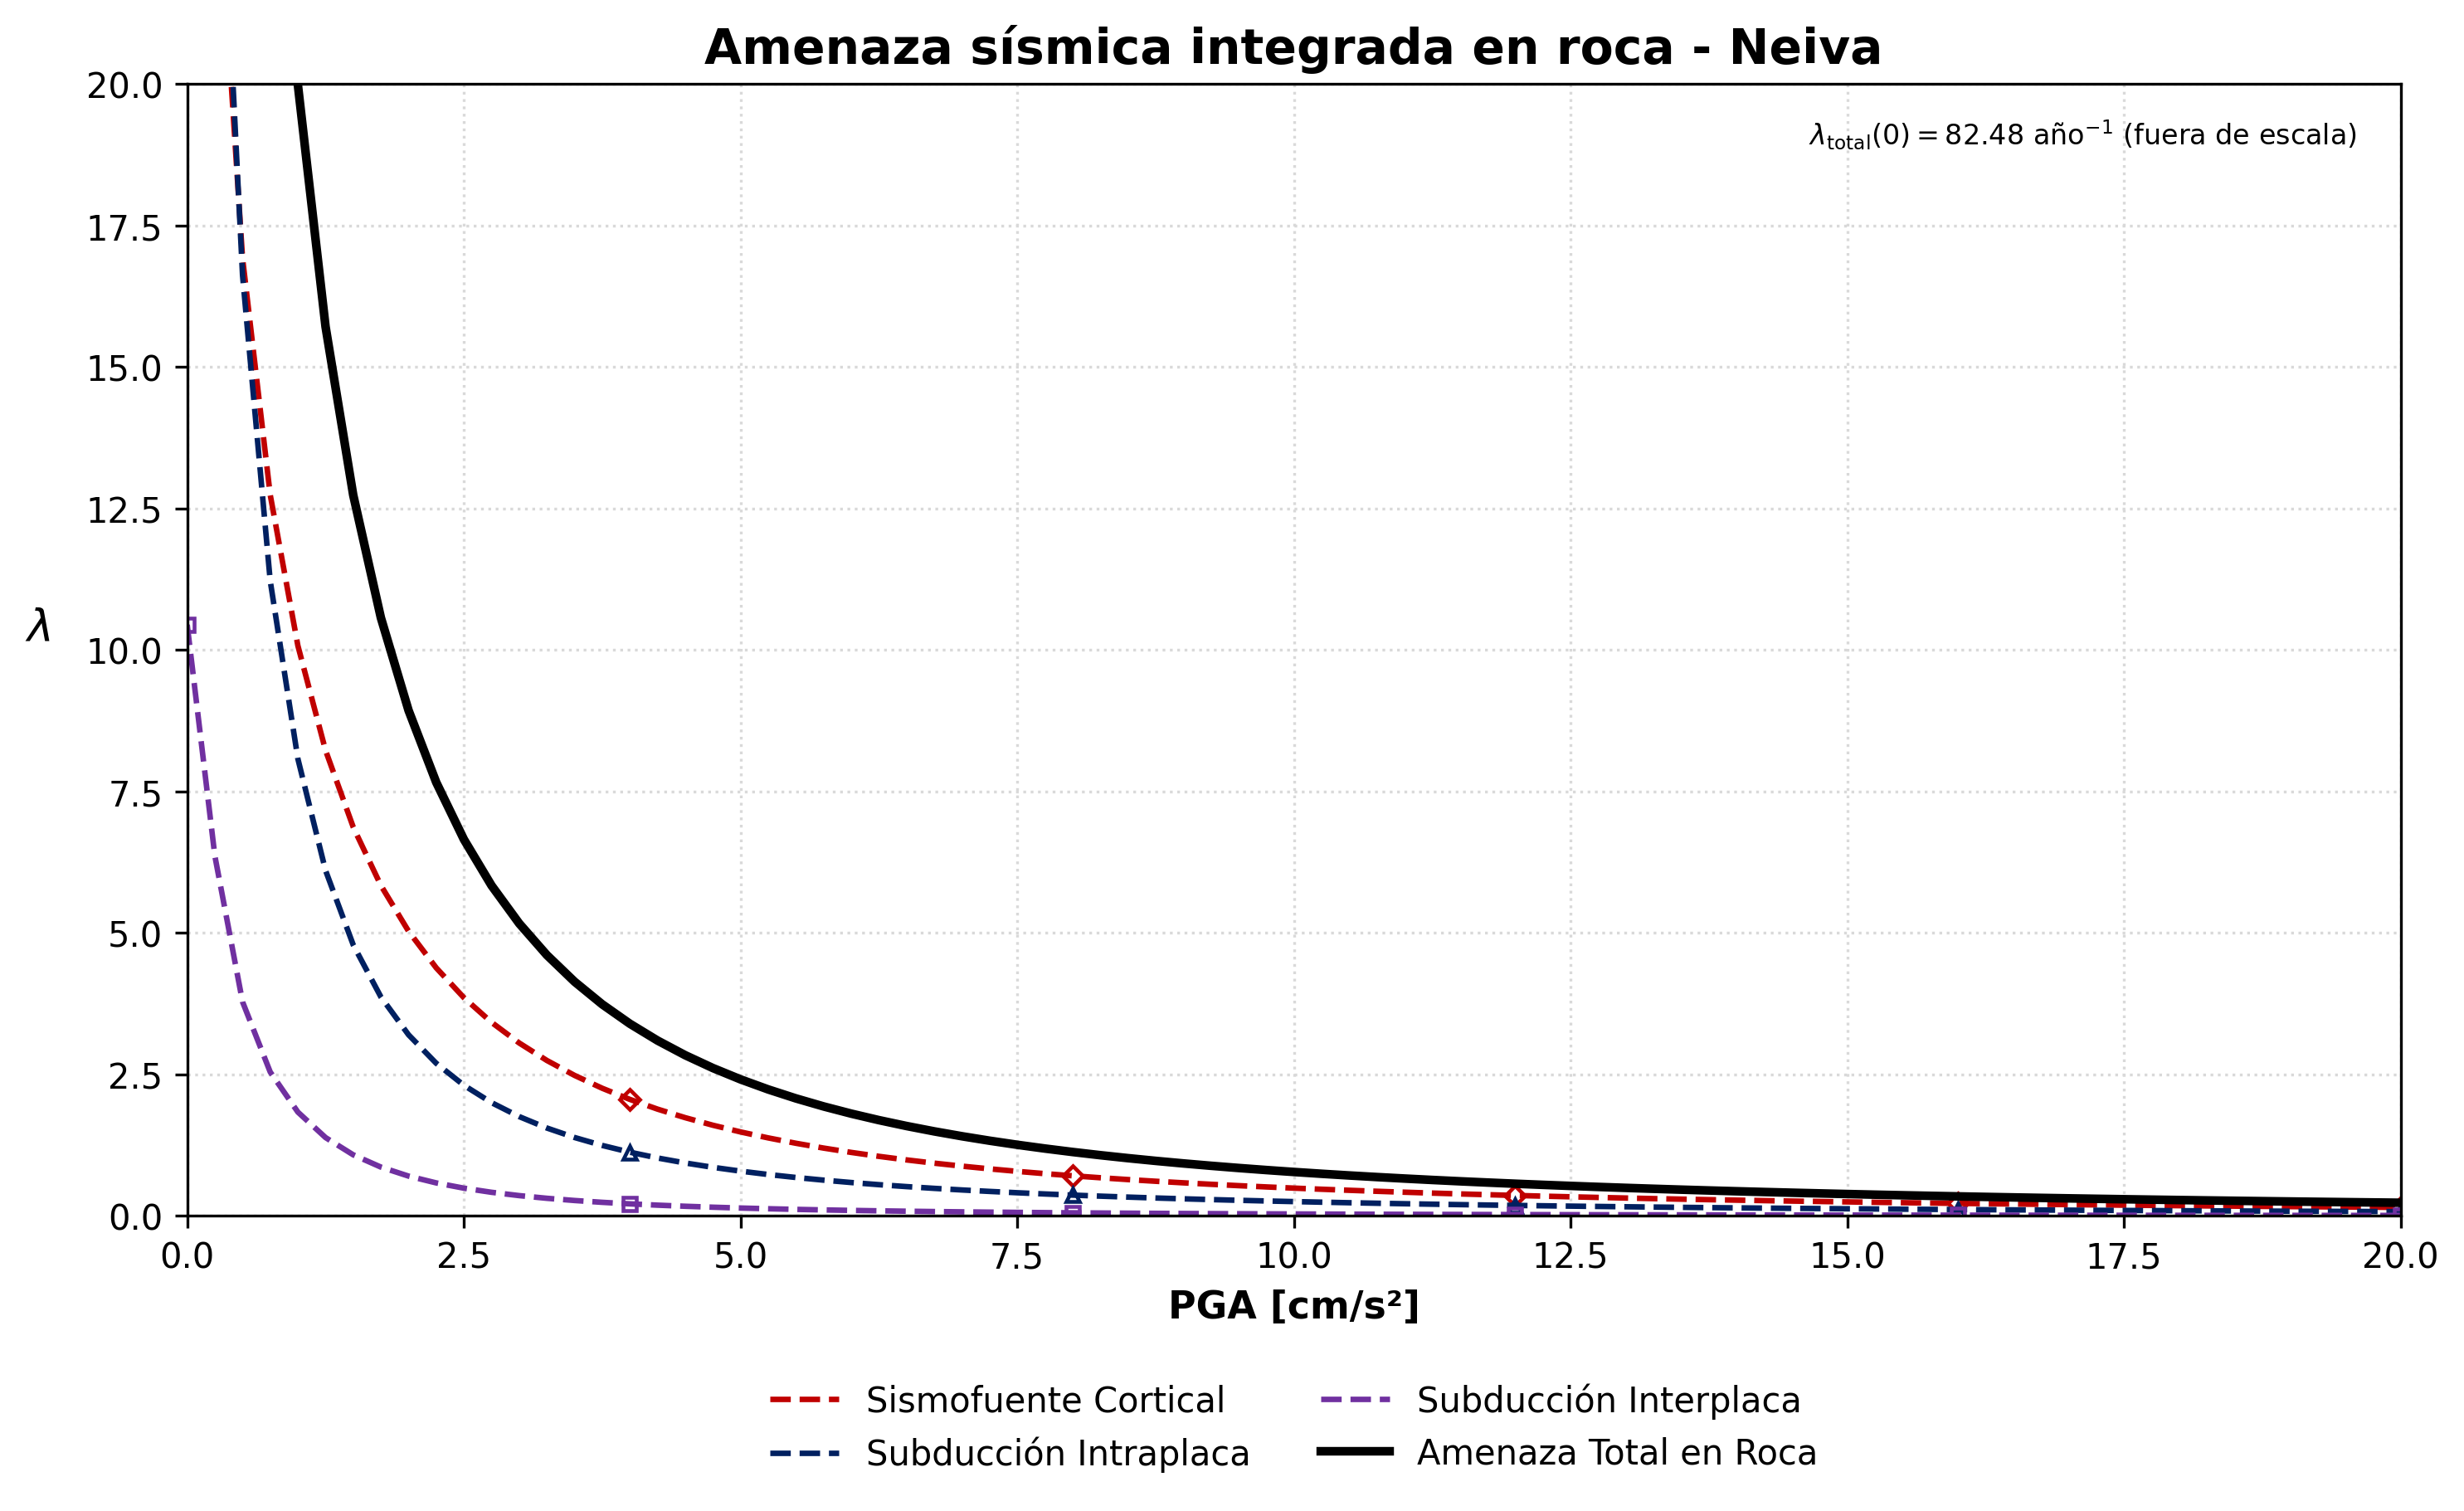
\includegraphics[width=0.68\linewidth]{../figuras/amenaza_sismica_neiva_figura8_local_aritmetica.png}
    \caption[Amenaza para aceleraciones bajas]{Amenaza para aceleraciones bajas. En Neiva se superan 5 cm/s$^2$ unas 2.4 veces por año y 20 cm/s$^2$ unas 0.23 veces por año.}
    \label{fig:amenaza-local-aritmetica}
\end{figure}

\subsection{Sismo esperado para 475 años}

Para saber qué sismos producen el PGA de 475 años, la tasa $\lambda=1/475$
se separa por fuente, magnitud y distancia (desagregación): cada término de
la suma anterior es el aporte de una fuente, una magnitud y un sismo del
catálogo (Figura~\ref{fig:desagregacion} y Tabla~\ref{tab:desagregacion}).

\begin{figure}[H]
    \centering
    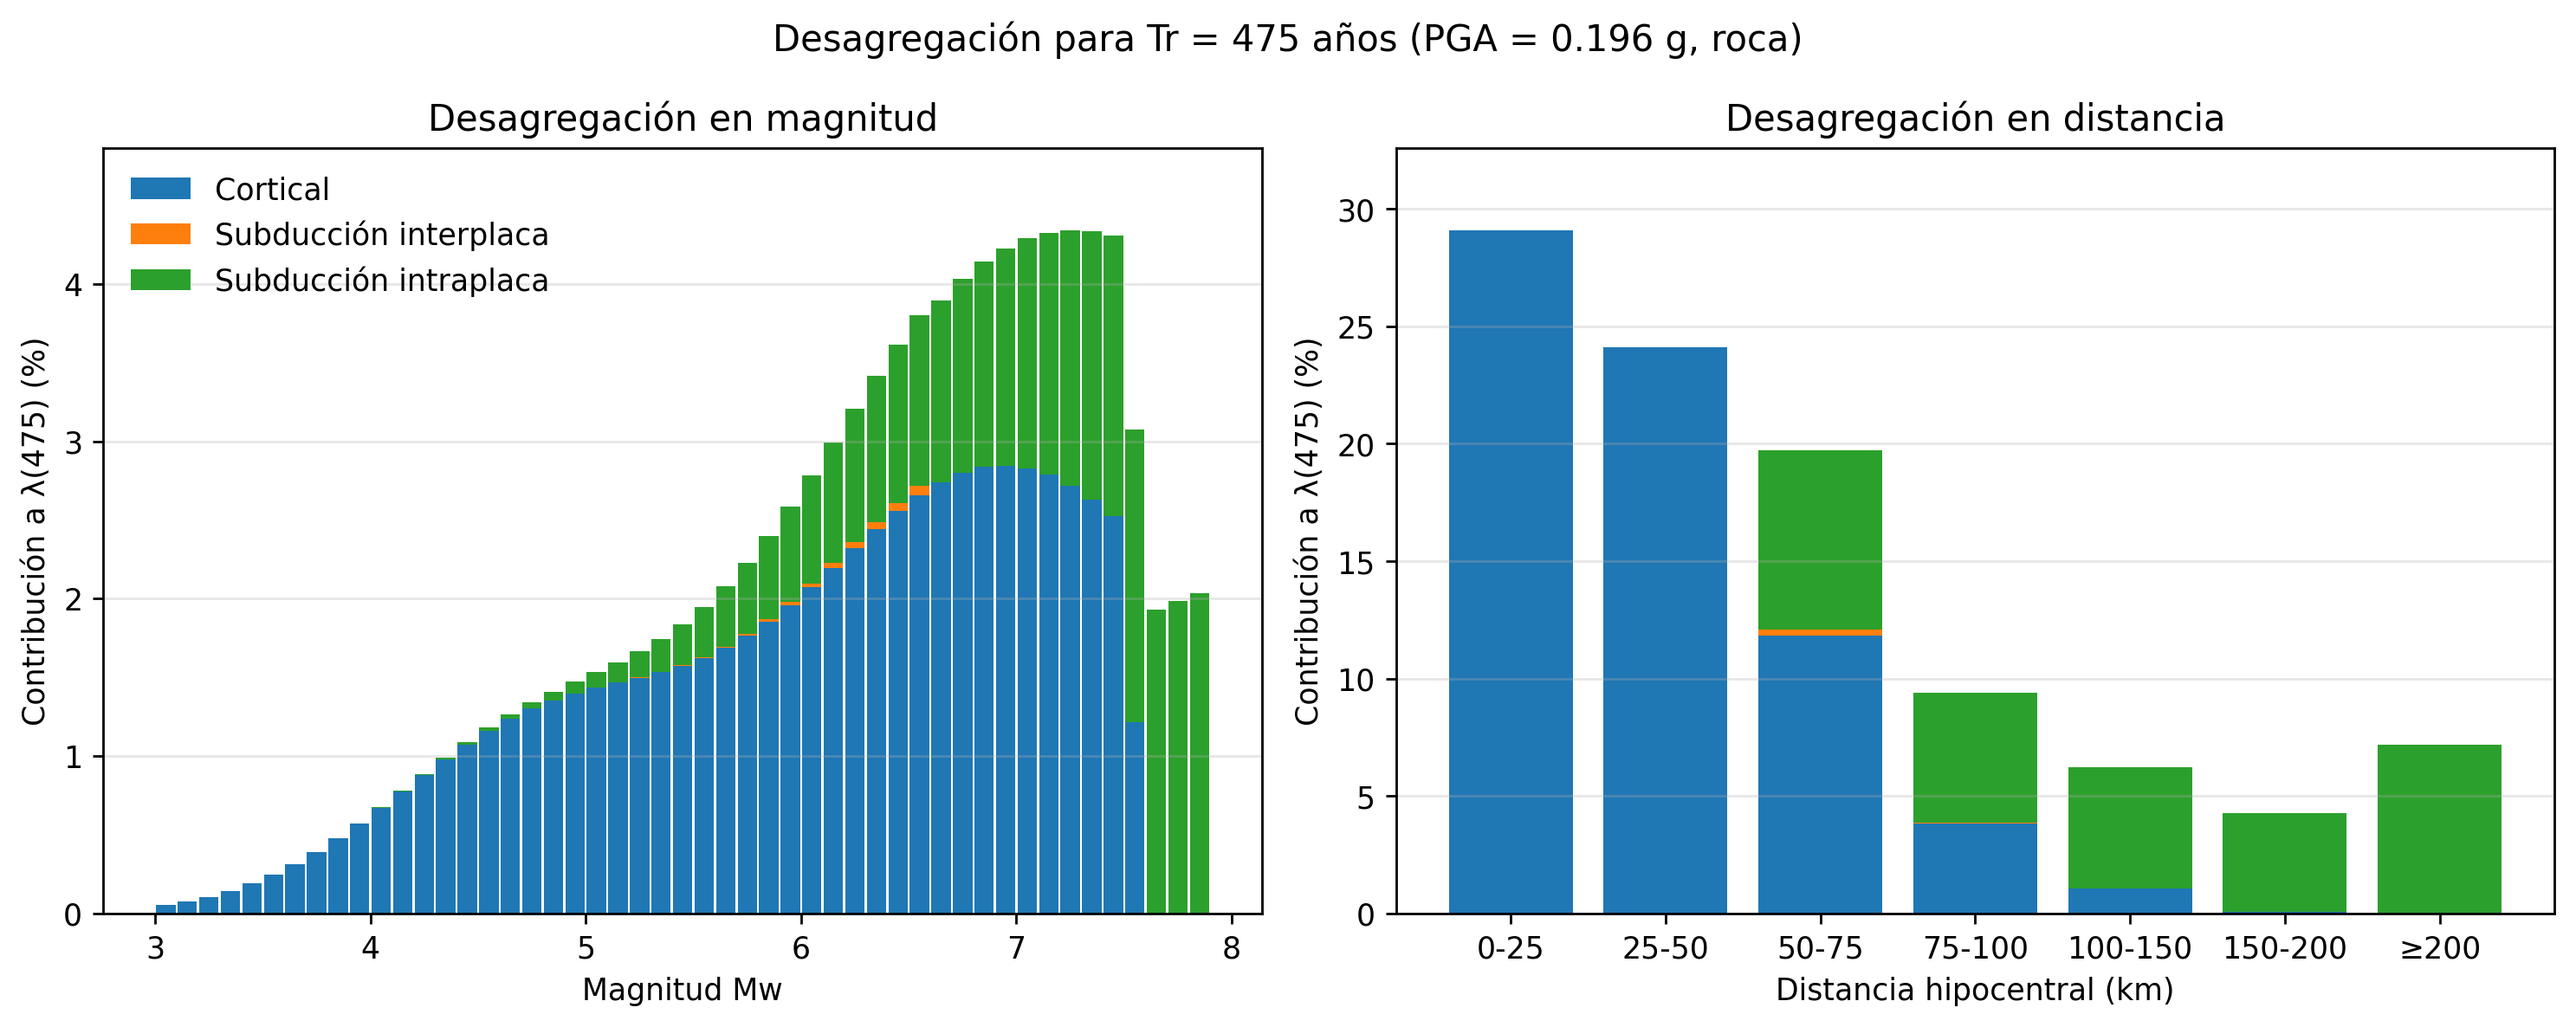
\includegraphics[width=0.9\linewidth]{../figuras/desagregacion_neiva_475.png}
    \caption[Desagregación de la amenaza de 475 años]{Desagregación de la amenaza de 475 años. La mitad del aporte viene de sismos a menos de 46 km del sitio.}
    \label{fig:desagregacion}
\end{figure}

\begin{table}[H]
\centering
\customtablecaption{Tabla 7}{Desagregación de la amenaza de 475 años.}
\label{tab:desagregacion}
\scriptsize
\begin{tabular}{lrrrrr}
\toprule
Fuente & Aporte (\%) & $M_w$ media & $X$ media (km) & $X$ mediana (km) & $h$ media (km) \\
\midrule
Cortical & 70.0 & 6.04 & 33 & 34 & 9 \\
Subducción interplaca & 0.3 & 6.23 & 71 & 72 & 9 \\
Subducción intraplaca & 29.7 & 6.94 & 132 & 110 & 95 \\
\midrule
Total & 100 & 6.31 & 63 & 46 & 35 \\
\bottomrule
\end{tabular}
\end{table}

La amenaza la controlan dos escenarios: un sismo cortical de
$M_w\approx6.0$ a unos 33 km (70\%) y un sismo intraplaca de $M_w\approx6.9$
a unos 130 km y 95 km de profundidad (30\%). La interplaca no influye
(0.3\%). Estos dos sismos, junto con el interplaca, son los sismos de
control del Paso 5.

\section{Paso 5: espectros de respuesta y espectro de aceleración}

\subsection{Espectros de respuesta en roca}

Se calculó el espectro de respuesta (5\% de amortiguamiento) del sismo de
control de cada fuente (Tabla~\ref{tab:desagregacion}), con una ecuación
según el tipo de fuente:
\begin{itemize}
    \item \textbf{Cortical: Sadigh et al. (1997)} \parencite{sadigh1997}, hecha
    para sismos corticales poco profundos:
    \begin{equation*}
    \ln S_a=C_1+C_2M+C_3(8.5-M)^{2.5}+C_4\ln\!\left[r+e^{C_5+C_6M}\right]+C_7\ln(r+2),
    \end{equation*}
    donde $S_a$ es la aceleración espectral en $g$, $M$ la magnitud
    momento, $r$ la distancia a la ruptura en km y $C_1$ a $C_7$ los
    coeficientes de cada periodo, tomados de la tabla de Sadigh et al.
    (1997) para roca y $M\leq6.5$. Para el sismo de control
    ($M_w\approx6.0$) la ruptura mide pocos kilómetros, así que $r$ se toma
    igual a la distancia hipocentral.
    \item \textbf{Subducción: Zhao et al. (2006)}, la misma ecuación del
    Paso 3 con los coeficientes de cada periodo. Sadigh no sirve para estas
    fuentes porque no tiene en cuenta la profundidad ni el tipo de fuente;
    el SGC también usa Zhao para subducción \parencite{sgc2018amenaza}.
\end{itemize}

\begin{table}[H]
\centering
\customtablecaption{Tabla 8}{Sismos de control y espectros de respuesta medianos.}
\label{tab:espectros-fuentes}
\scriptsize
\begin{tabular}{llrrrrr}
\toprule
Fuente & Ecuación & $M_w$ & $X$ (km) & PGA (g) & $S_{a,\max}$ (g) & $T$ del máximo (s) \\
\midrule
Cortical & Sadigh et al. (1997) & 6.0 & 33 & 0.061 & 0.138 & 0.20 \\
Subducción interplaca & Zhao et al. (2006) & 6.2 & 71 & 0.026 & 0.062 & 0.15 \\
Subducción intraplaca & Zhao et al. (2006) & 6.9 & 132 & 0.069 & 0.169 & 0.15 \\
\bottomrule
\end{tabular}
\end{table}

\begin{figure}[H]
    \centering
    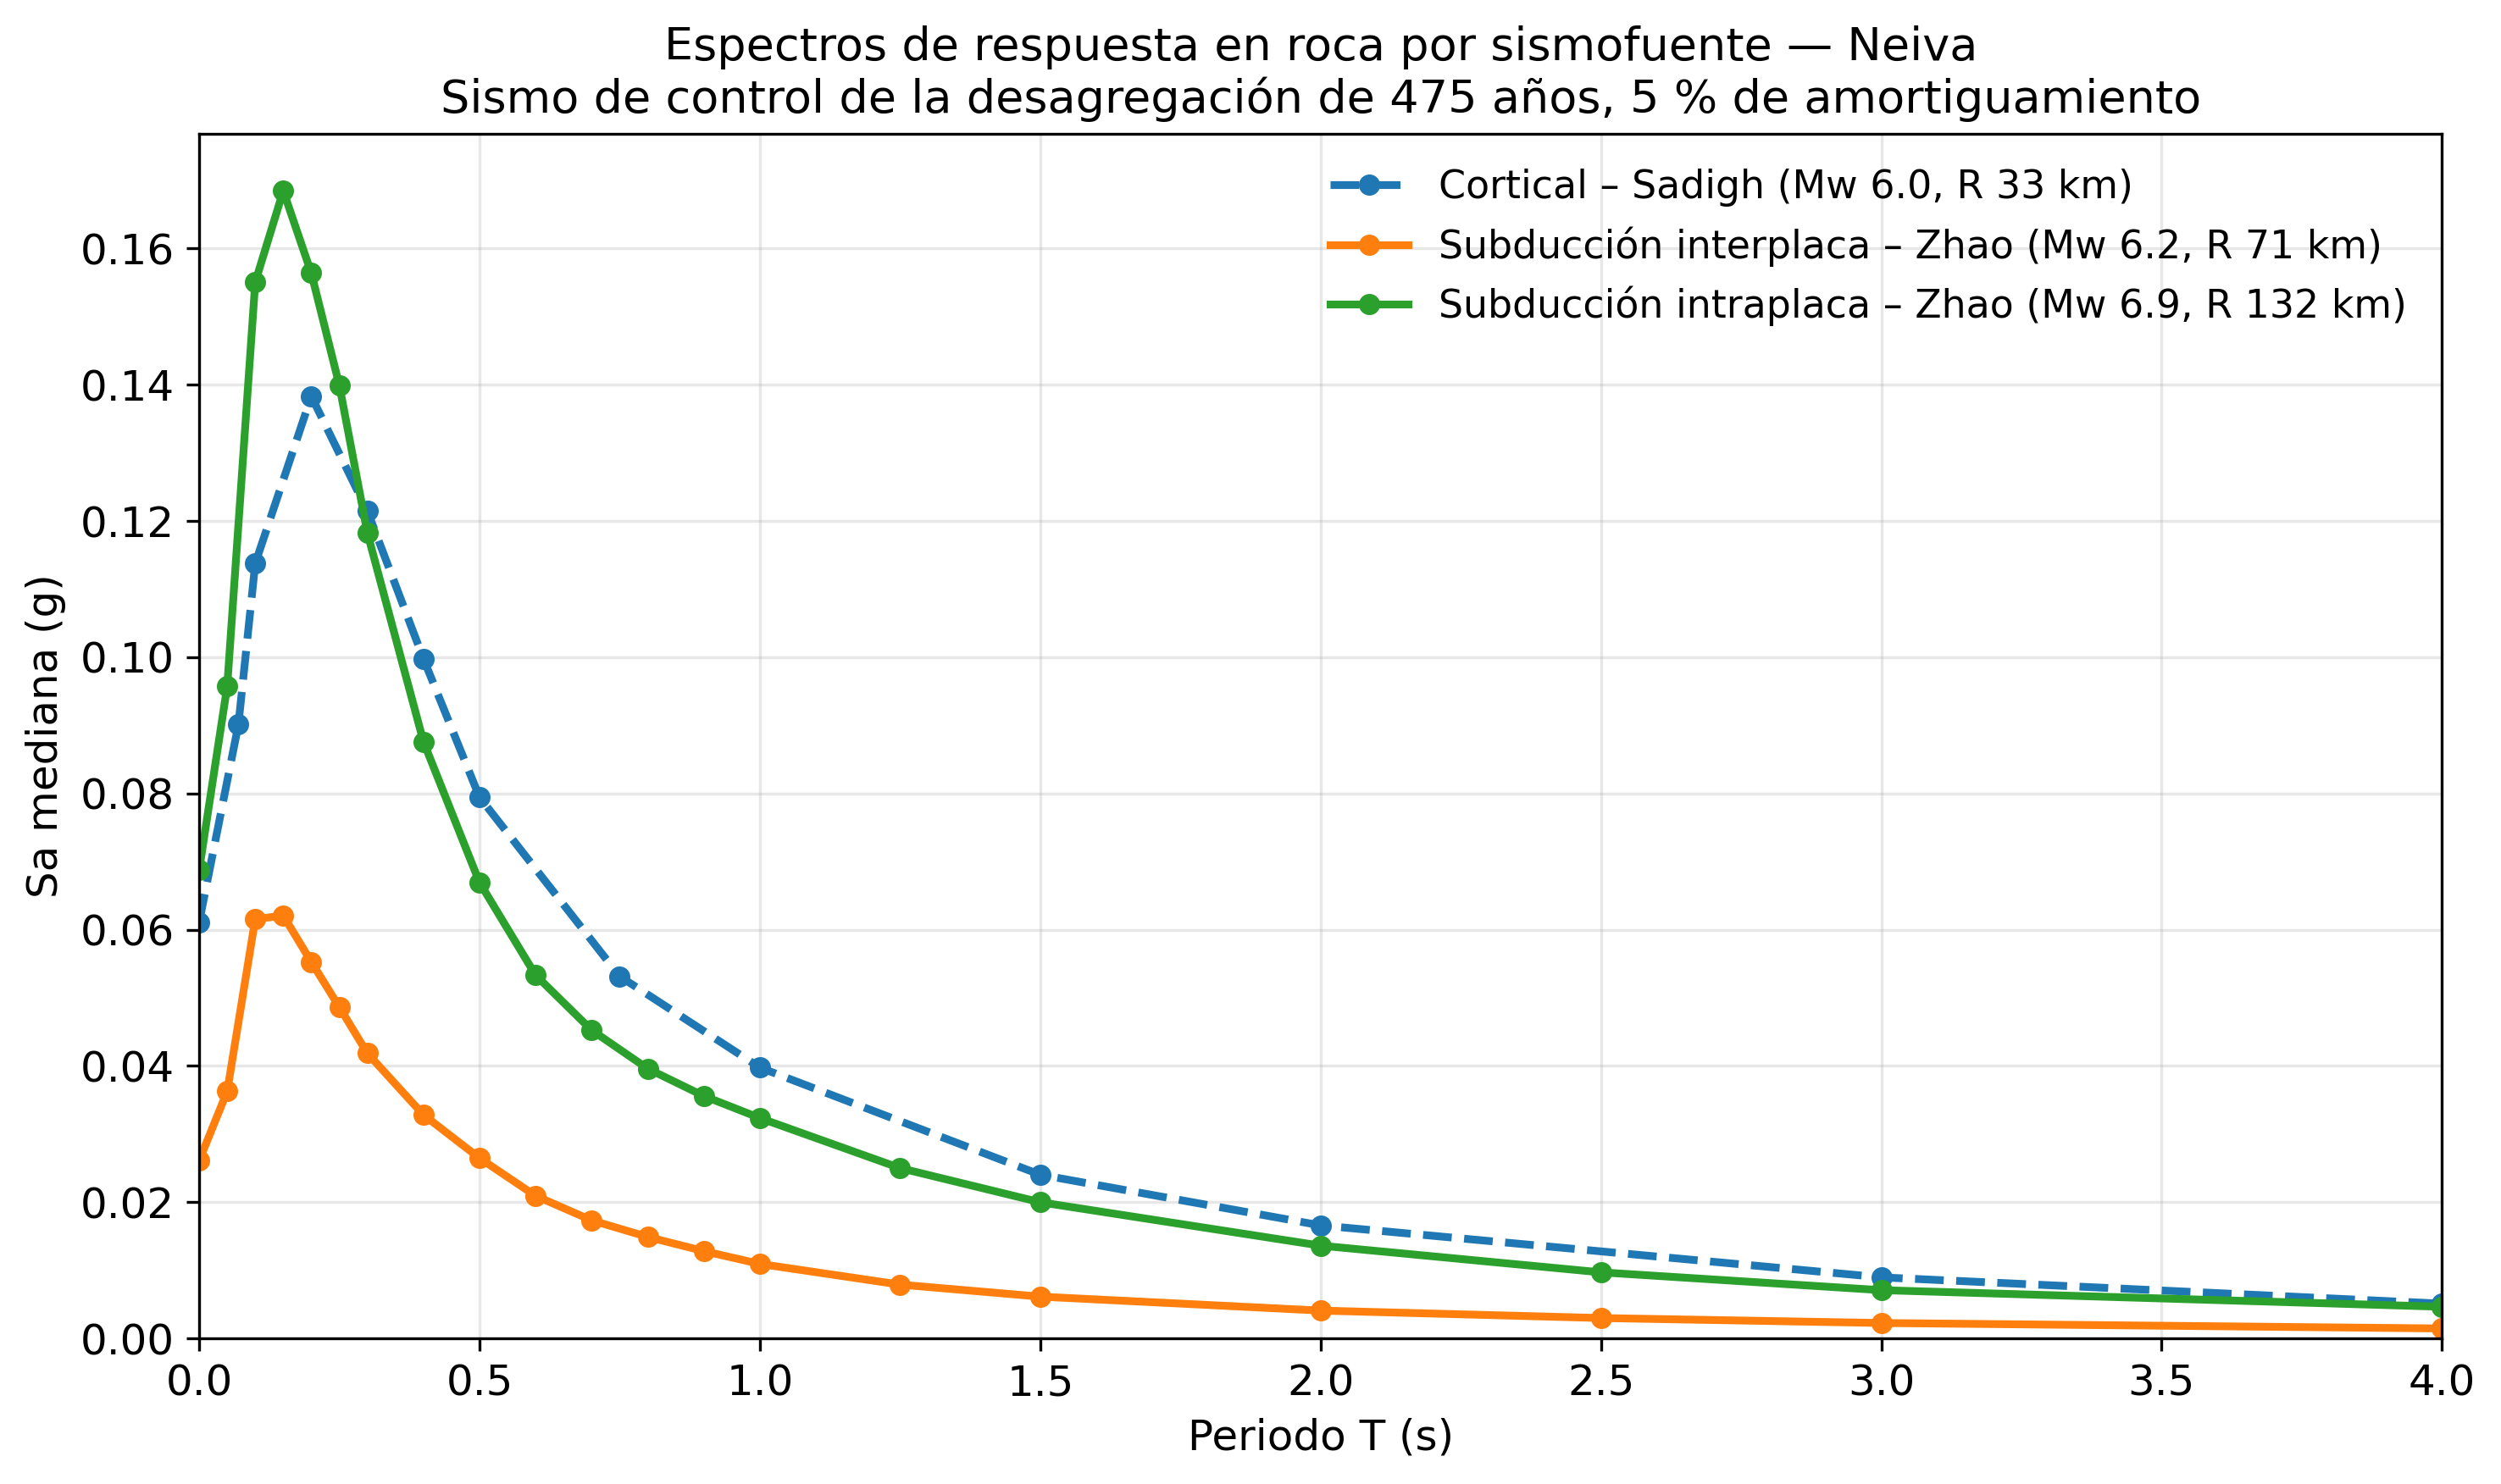
\includegraphics[width=0.74\linewidth]{../figuras/espectros_respuesta_fuentes_neiva.png}
    \caption[Espectros de respuesta en roca por fuente]{Espectros de respuesta en roca por fuente. La intraplaca domina hasta 0.25 s y la cortical en periodos mayores.}
    \label{fig:espectros-fuentes}
\end{figure}

En las tres fuentes el pico del espectro es de 2.3 a 2.5 veces el PGA,
dentro del rango de 2.1 a 2.7 que proponen Newmark y Hall para 5\% de
amortiguamiento \parencite{newmark1982}. El pico ocurre en periodos cortos
(0.15 a 0.2 s). La interplaca da valores mucho menores porque su sismo de
control es pequeño y lejano.

\subsection{Espectro de aceleración en roca}

Los espectros de la Tabla~\ref{tab:espectros-fuentes} son medianos (PGA de
0.03 a 0.07 $g$), mientras que el nivel de 475 años es más fuerte
(0.196 $g$). Por eso se conserva la forma de cada espectro y se escala al
PGA de 475 años:
\begin{equation*}
S_{a,i}^{\mathrm{esc}}(T)=\mathrm{PGA}_{475}\,\frac{S_{a,i}(T)}{\mathrm{PGA}_i},
\end{equation*}
donde $S_{a,i}(T)$ y $\mathrm{PGA}_i$ son el espectro y el PGA medianos de
la fuente $i$. El espectro de aceleración tiene la forma de la NSR-10
(rampa, meseta y caída con $1/T$) y se trazó por encima de los tres
espectros escalados:
\begin{equation*}
S_a(T)=
\begin{cases}
\mathrm{PGA}+\left(S_{a,\max}-\mathrm{PGA}\right)\dfrac{T}{T_0}, & T<T_0,\\[6pt]
S_{a,\max}, & T_0\le T\le T_C,\\[6pt]
S_{a,\max}\,\dfrac{T_C}{T}, & T>T_C,
\end{cases}
\end{equation*}
donde $S_{a,\max}$ es el pico más alto de los espectros escalados y $T_0$ y
$T_C$ son los periodos con los que la rampa y la caída cubren a todos. El
resultado es $\mathrm{PGA}=0.196\,g$, $S_{a,\max}=0.481\,g$, $T_0=0.10$ s y
$T_C=0.28$ s. La intraplaca define la meseta y la cortical la caída.

\begin{figure}[H]
    \centering
    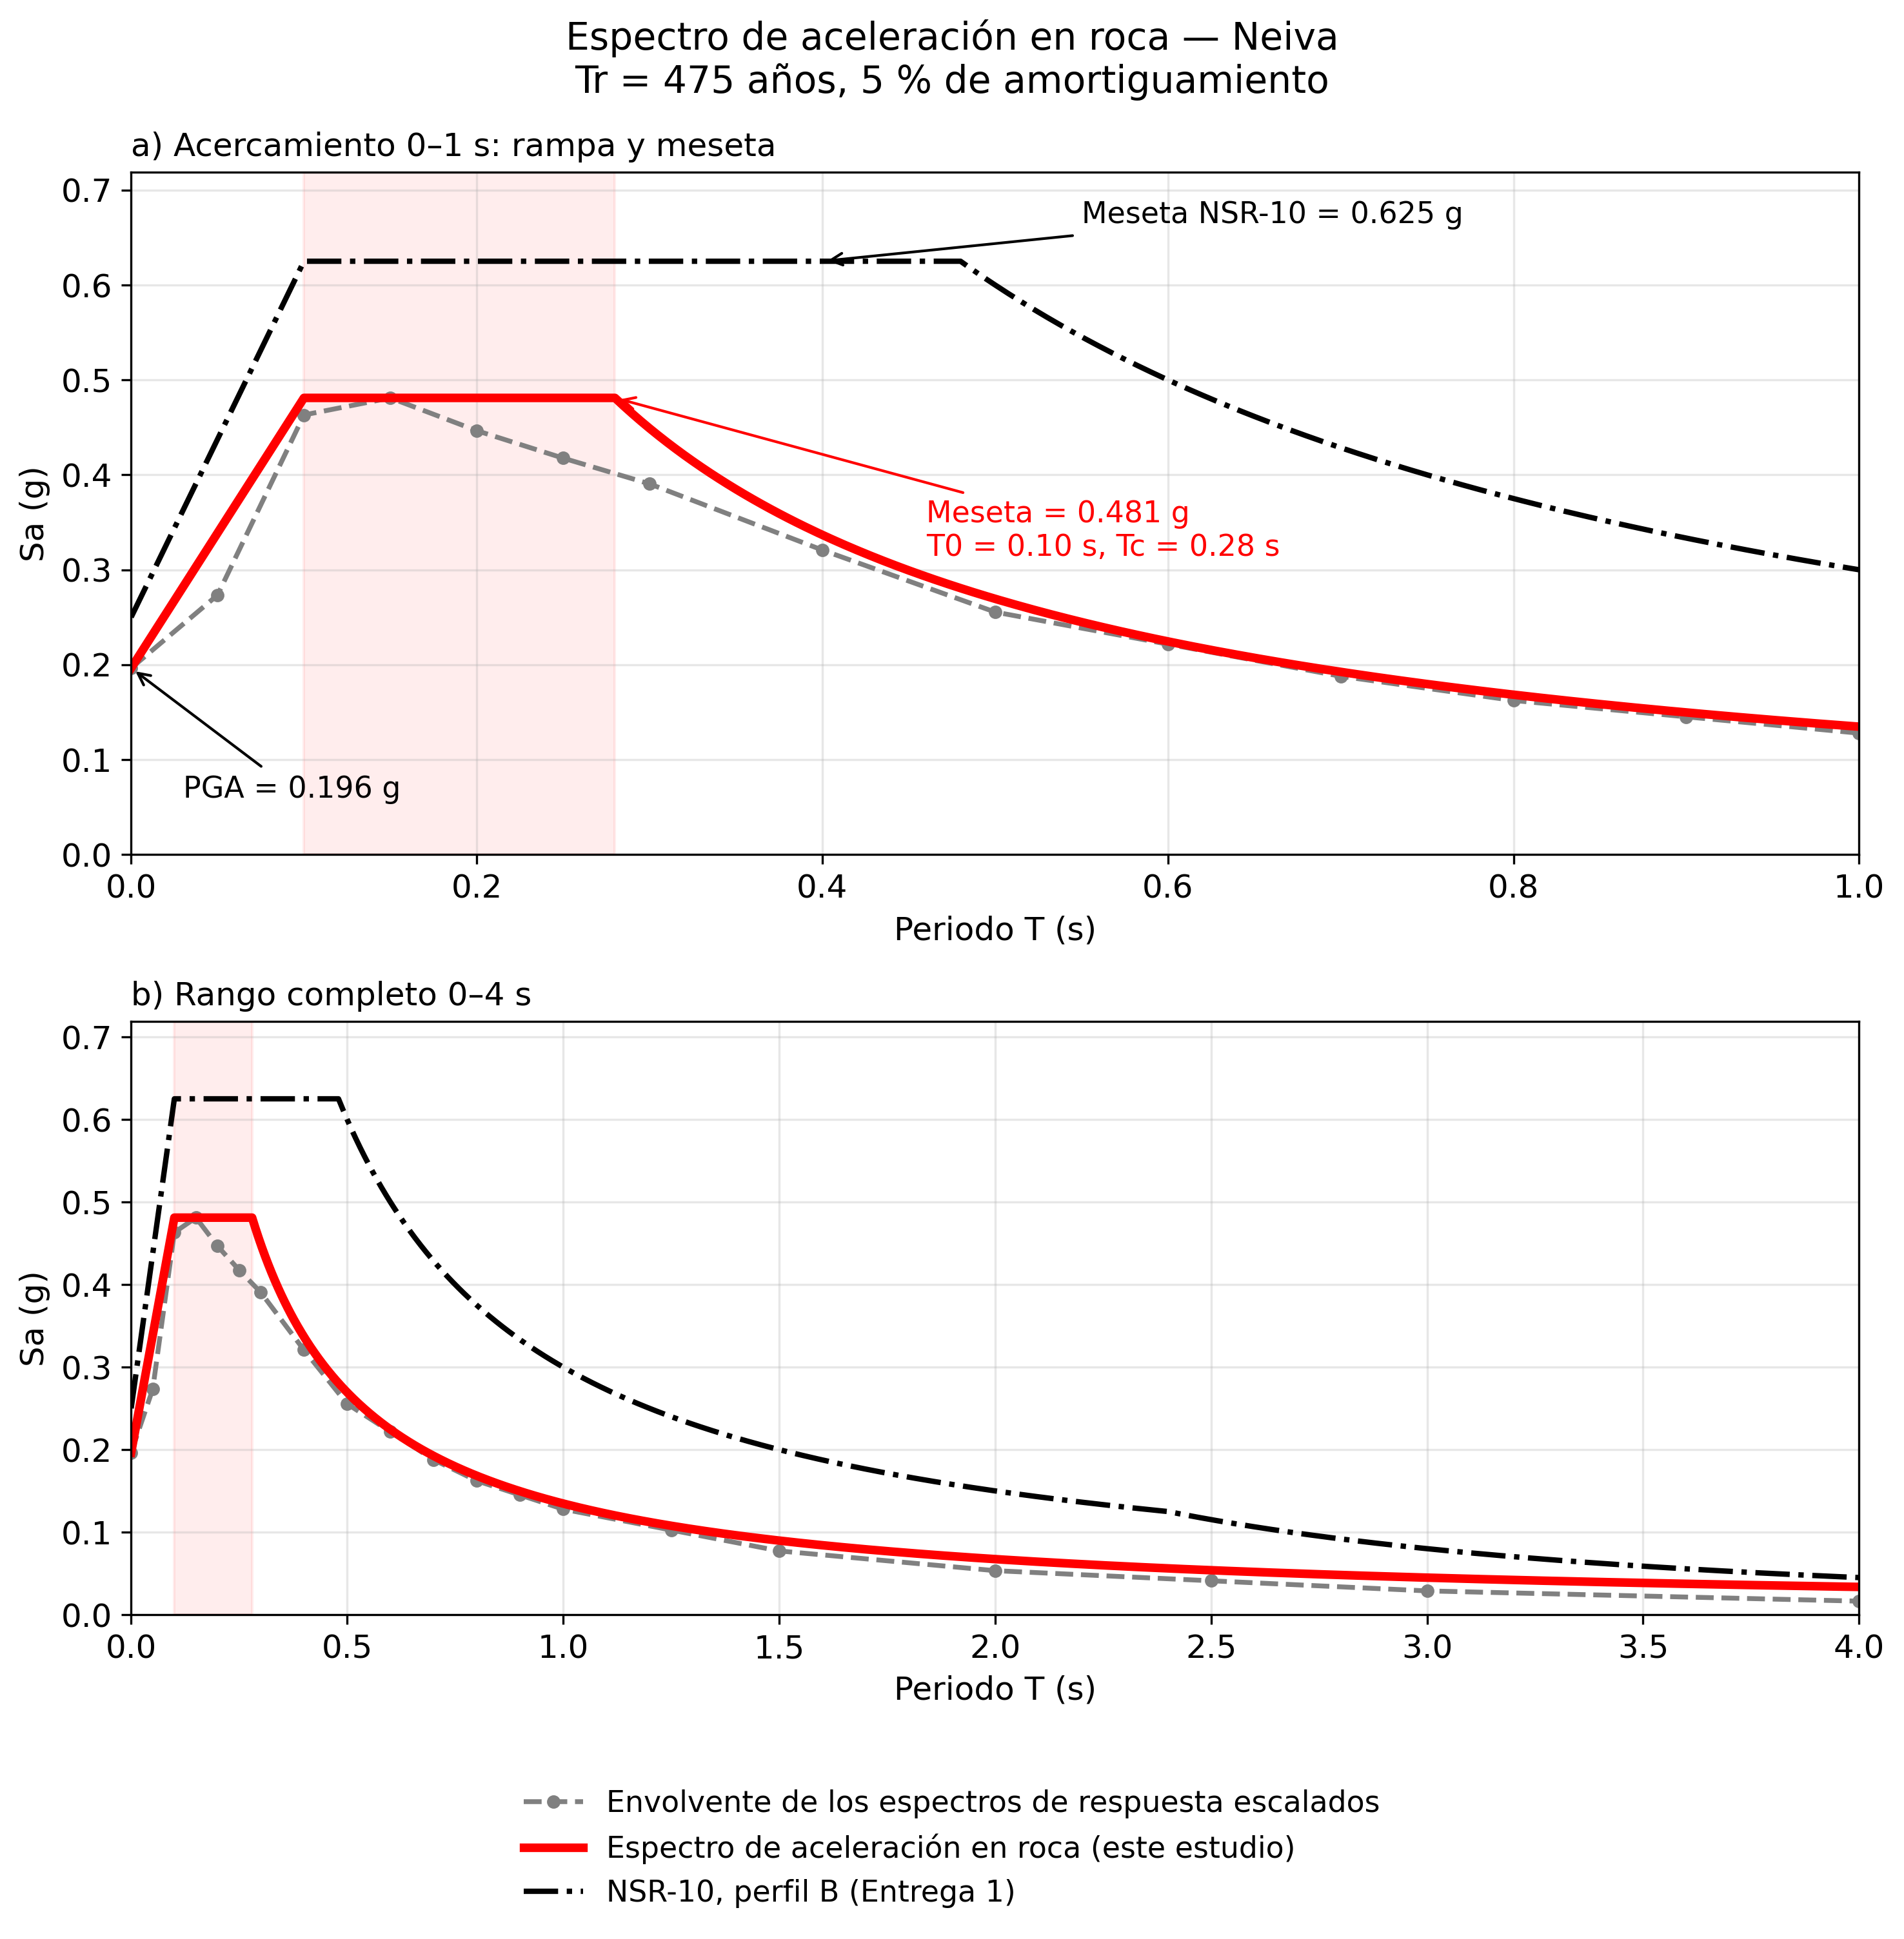
\includegraphics[width=0.95\linewidth,height=0.5\textheight,keepaspectratio]{../figuras/espectro_diseno_roca_neiva.png}
    \caption[Espectro de aceleración en roca]{Espectro de aceleración en roca para 475 años, comparado con el espectro NSR-10 en roca de la Entrega 1. El espectro obtenido queda por debajo de la norma en todos los periodos.}
    \label{fig:espectro-diseno}
\end{figure}

\begin{table}[H]
\centering
\customtablecaption{Tabla 9}{Comparación con el espectro NSR-10 en roca.}
\label{tab:comparacion-nsr10}
\scriptsize
\begin{tabular}{lrr}
\toprule
Parámetro & Este estudio & NSR-10 (Entrega 1) \\
\midrule
PGA (g) & 0.196 & 0.25 \\
Meseta $S_{a,\max}$ (g) & 0.481 & 0.625 \\
$T_0$ (s) & 0.10 & 0.10 \\
$T_C$ (s) & 0.28 & 0.48 \\
$A_a$ equivalente ($S_{a,\max}/2.5$) & 0.19 & 0.25 \\
\bottomrule
\end{tabular}
\end{table}

La meseta obtenida es un 23\% menor que la de la NSR-10 y termina antes
(0.28 s frente a 0.48 s), así que la diferencia crece en periodos
intermedios. La NSR-10 usa un catálogo y un modelo de fuentes más amplios;
para diseño sigue rigiendo la norma.

\section{Conclusiones}

\begin{itemize}
    \item El catálogo regional de 260 km tiene 2\,691 sismos con $M_w\geq3.0$
    en tres fuentes. La cortical es la más activa en magnitudes bajas y la
    intraplaca tiene la mayor proporción de sismos grandes ($b=0.821$).
    \item El PGA en roca para 475 años es 0.196 $g$ (192.6 cm/s$^2$), el 79\%
    del $A_a=0.25$ de la NSR-10. Para 100, 975 y 2\,475 años es 0.101, 0.260
    y 0.366 $g$.
    \item La amenaza la controla la fuente cortical (70\%), con un sismo de
    $M_w\approx6.0$ a unos 33 km, seguida de la intraplaca (30\%), con un
    sismo de $M_w\approx6.9$ a unos 130 km y 95 km de profundidad. La
    subducción interplaca no influye.
    \item El resultado depende de la magnitud máxima: al variarla en
    $\pm0.5$, el PGA de 475 años queda entre 0.177 y 0.213 $g$.
    \item Los espectros de respuesta tienen su pico entre 0.15 y 0.2 s, con
    amplificaciones de 2.3 a 2.5 veces el PGA.
    \item El espectro de aceleración en roca tiene PGA de 0.196 $g$ y meseta
    de 0.481 $g$ entre 0.10 y 0.28 s. Queda por debajo del espectro NSR-10 en
    todos los periodos.
\end{itemize}

\section{Limitaciones y recomendaciones}

\begin{itemize}
    \item El catálogo cubre 109 años y tiene pocos sismos grandes; la
    magnitud máxima se fijó sin datos geológicos y el resultado es sensible
    a ella (Tabla~\ref{tab:sensibilidad-pga}).
    \item Las ecuaciones de Zhao (Japón) y Sadigh (California) no se
    calibraron con registros colombianos, y se usó una sola ecuación por
    fuente. El SGC combina varias en un árbol lógico; se recomienda incluir
    al menos una segunda ecuación por tipo de fuente.
    \item Las fuentes se representan con la ubicación de los sismos
    registrados, no con la geometría de las fallas; las zonas sin sismicidad
    reciente pueden quedar subrepresentadas.
    \item Sin mecanismos focales se desactivó el término de falla inversa de
    Zhao. Si se confirmara un mecanismo inverso, la amenaza cortical
    aumentaría.
    \item Todos los resultados son en roca. Los suelos de Neiva pueden
    amplificar el movimiento; eso se evaluará en el análisis de respuesta de
    sitio.
    \item Como el PGA y el espectro obtenidos son menores que los de la
    NSR-10, se recomienda compararlos con el modelo nacional del SGC
    \parencite{sgc2018amenaza} antes de usarlos para algo distinto a este
    ejercicio académico.
\end{itemize}

\section*{Referencias}
\small
\printbibliography[heading=none]

\end{document}
